\chapter{Literature Review}
\label{chap: 2}

\section{Scope and Goal for literature review}
\label{sect: 2.1scope}

This chapter provides an overview of the current knowledge and available literature on ML-accelerated CFD simulations. As a start, \autoref{sect: 2.2turbflows} explains the most frequently implemented methods in which turbulent simulations can be resolved. Next \autoref{sect: 2.5ML enhancing} will introduce how current advances in machine learning and artificial intelligence are being incorporated in the current CFD landscape.  

\section{Turbulent flows: simulation and modelling}
\label{sect: 2.2turbflows}

Fluid dynamics is governed by a set of coupled partial differential equations (PDE's) called the Navier-Stokes Equations (NSE). These equations are based on the assumptions of conservation of mass and momentum. These equations are shown in \ref{eq: navier-stokes} in \textit{Einstein notation} \cite{Turbulence}. Note that the equations seen in \ref{eq: navier-stokes} display the governing equations of a fluid of which we have assumed a constant density, which means that density $\rho$ is a material property and not something that needs to be solved for.

\begin{subequations} \label{eq: navier-stokes}

    % Continuity
    \begin{equation} \label{eq: continuity}
    \begin{aligned}
    \frac{\partial u_i}{\partial x_i} &= 0
    \end{aligned}
    \end{equation}

    % Momentum
    \begin{equation} \label{eq: momentum}
    \begin{aligned}
   \underbrace{ \frac{\partial u_i}{\partial t} }_{\text{Local acceleration}}
+ 
\underbrace{ u_j \frac{\partial u_i}{\partial x_j} }_{\text{Convective term}}
= 
\underbrace{ -\frac{1}{\rho} \frac{\partial p}{\partial x_i} }_{\text{Pressure gradient}}
+ 
\underbrace{ \nu \frac{\partial^2 u_i}{\partial x_j \partial x_j} }_{\text{Viscous diffusion}}
+ 
\underbrace{ g_i }_{\text{Body forces}}
    \end{aligned}
    \end{equation}
\end{subequations}

Where $u$ is the 3-dimensional velocity vector, $x$ is the position vector, $p$ is the pressure in the fluid, $\nu$ is the kinematic viscosity of the fluid, $g$ is the gravitational constant, $t$ is time and finally the subscripts $i$ and $j$ indicate spatial directions.

These equations have proven to be a tough fluid dynamics challenge and have yet to be solved analytically. Due to their non-linearity and strong coupling, they display complex behaviour. This behaviour mainly arises from the non-linear convective term in the momentum equation. This fact is particularly pronounced for high Reynolds number flows, where small-scale turbulent structures dominate \cite{Turbulence}. In current mathematics, solutions to the most fundamental questions regarding the NSE remain elusive. Questions such as: do solutions exist, and are they unique \cite{clay_navierstokes}? It is due to this complexity and lack of understanding that the Clay Mathematics Institute has listed the NSE as one of the 7 Millennium Problems. Because no analytical solution exists, engineers and researchers must discretise, model, and make assumptions about various parts of the NSE to obtain numerical solutions to these equations. 

\subsection{DNS}
One way to evaluate the NSE is through a Direct Numerical Simulation (DNS). A DNS aims to capture all length and timescales of a turbulent flow directly, without modelling and without further assumptions. Furthermore, DNS must accurately resolve the temporal resolution of the turbulent flow it aims to simulate. Following Kolmogorov's microscale hypothesis \cite{Kolmogorov1941} and the two-point correlation function \cite{Pope2000}, the smallest and largest turbulent length scales can be obtained, respectively. Using these length scales, the mesh spacing and mesh dimensions can be determined; this way, all relevant length scales can be represented in the turbulent flow field without resorting to modelling. These length scales are strongly correlated to the Reynolds numbers, which is the ratio of inertial forces and viscous forces. 

\begin{equation}\label{eq: Reynoldsnr}
    Re = \frac{\text{Inertial forces}}{\text{Viscous forces}}= \frac{u l}{\nu}
\end{equation}

Where $u$ is the flow velocity and $l$ is the characteristic length. At large Reynolds numbers, turbulent flows exhibit a wide range of scales, where the smallest turbulent length scales become progressively smaller as $Re$ increases. This means that for a high $Re$ DNS, a very fine mesh would need to be generated. 

In fact, when following Kolmogorov in assuming the smallest scales of turbulence are universal and isotropic, the total number of grid points (degrees of freedom) required for a DSN scales with $Re^{9/4}$ \cite{Coleman2010}. Factoring in the necessary change in timestep to maintain a constant CFL number, the total computational effort for DNS would be equal to $\mathcal{O}(Re^3)$ \cite{Coleman2010}. This extensive computational requirement makes DNS highly accurate but prohibitively expensive for general practical use. However, it remains indispensable for fundamental turbulence research due to its ability to provide complete knowledge of the flow without empirical approximations.


\subsection{RANS}
One way to reduce the computational cost of numerical simulations of the NSE was stipulated by \textcite{Reynolds1895} in 1895. In this work, he proposed decomposing the instantaneous velocity into two distinct parts: the time-averaged part and the fluctuating part. 

\begin{equation}\label{eq: ReDecompose}
    u_i = \langle u_i \rangle + u_i'
\end{equation}

% \begin{wrapfigure}{r}{0.45\textwidth}
% \vspace{-1em}
%     \centering
%     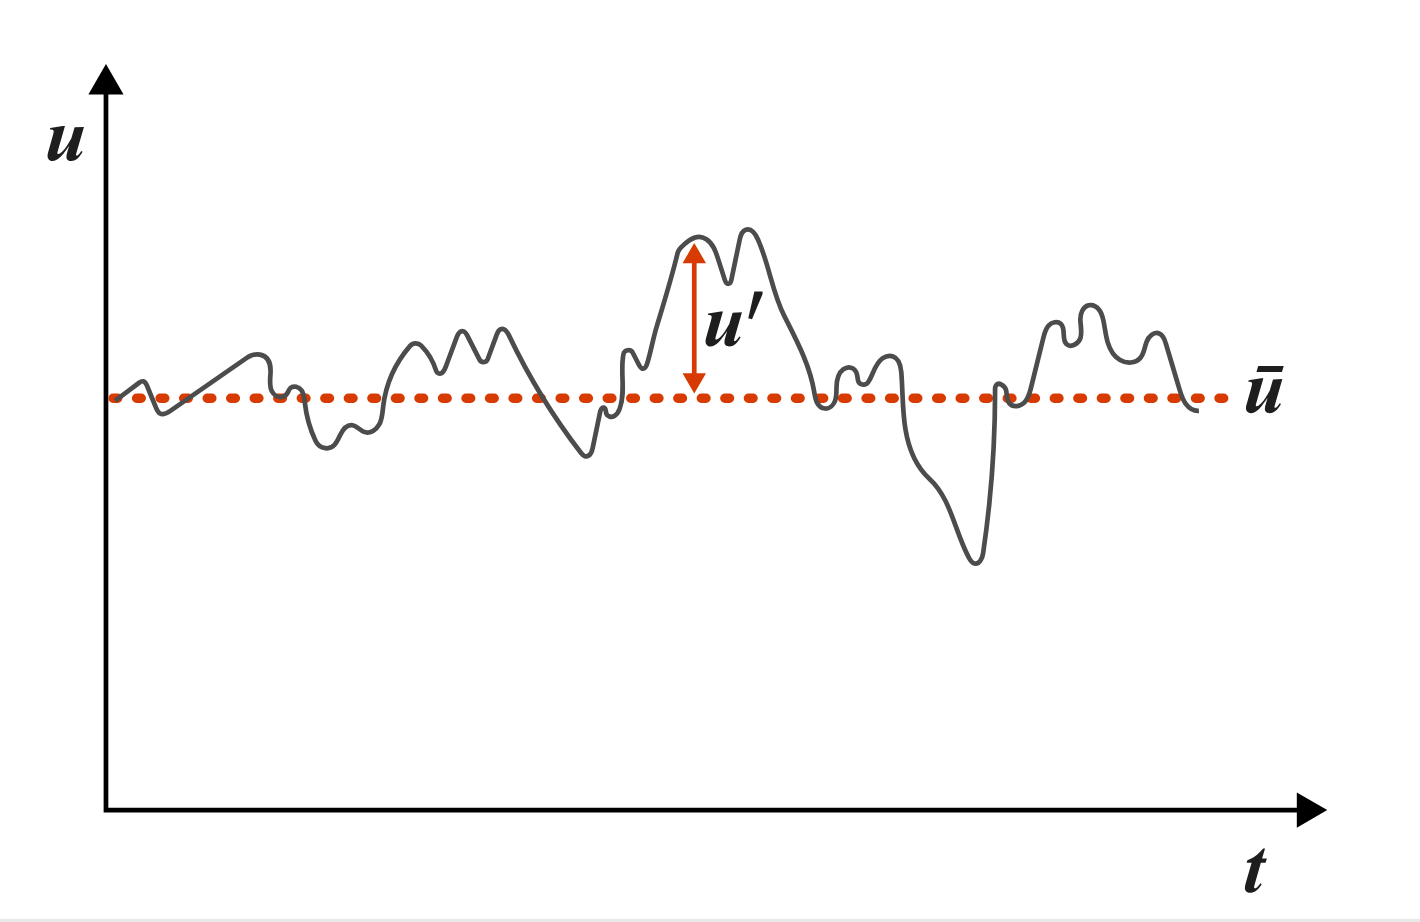
\includegraphics[width=\linewidth]{figures/Literature review/RANS.png}
%     \caption{Schematic of the Reynolds decomposition for incompressible flow: the instantaneous velocity $u(t)$ (solid line) is split into its time‐averaged mean $\overline{u}$ (dashed red line) and the fluctuation $u'(t)=u(t)-\overline{u}$. Adapted from \cite{Altair2021RANS}}    
%   \label{fig: rans}
%   \vspace{-1em}
% \end{wrapfigure}


% \noindent
% \begin{minipage}[c]{0.35\textwidth}
%   \begin{equation}
%     u_i = \langle u_i \rangle + u_i'
%     \label{eq: ReDecompose}
%   \end{equation}
% \end{minipage}\hfill
% \begin{minipage}[c]{0.65\textwidth}
%   \centering
%   % 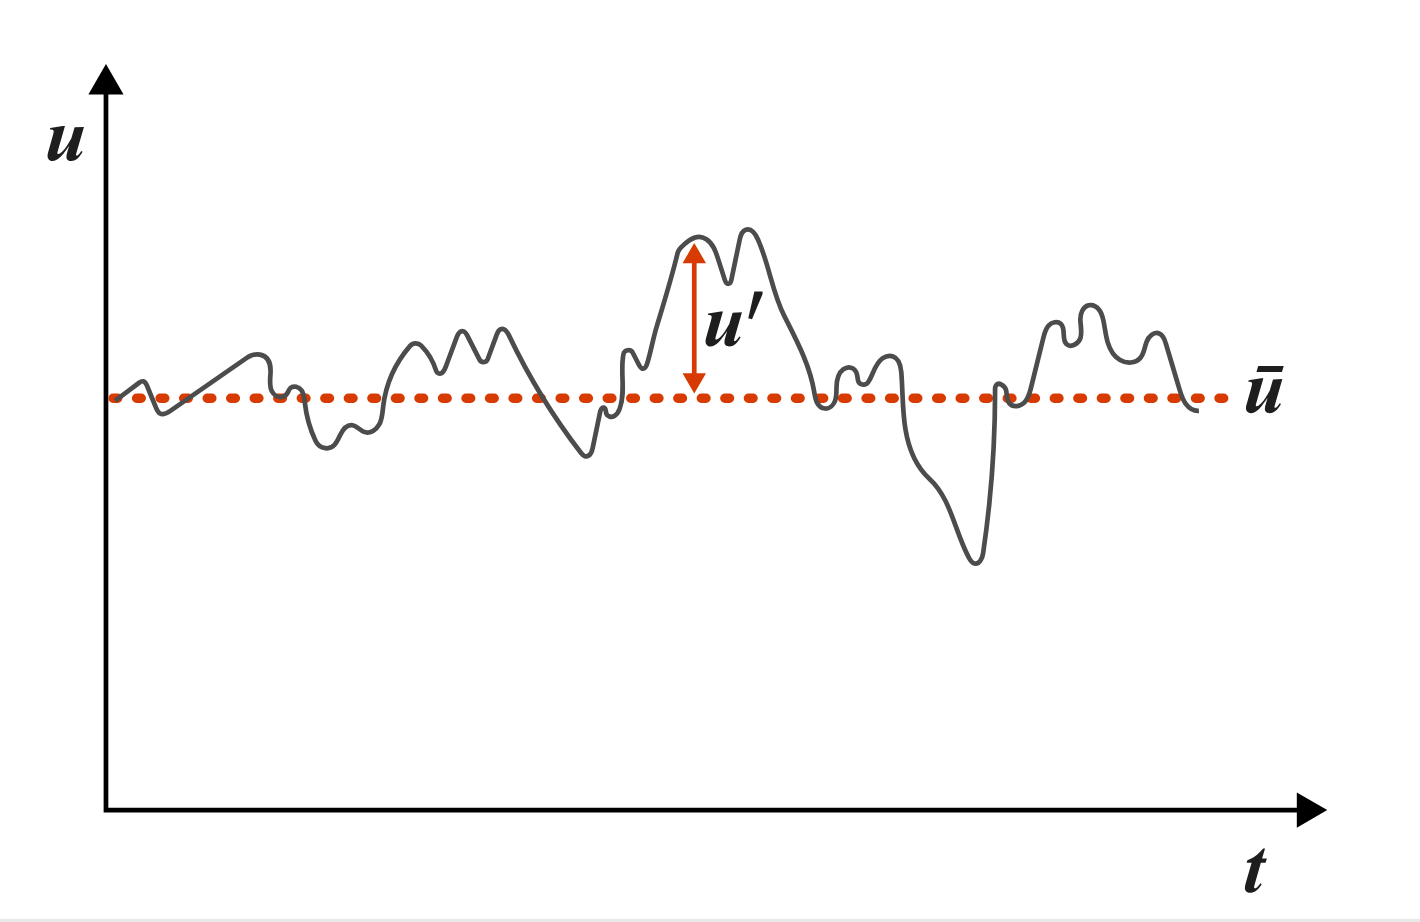
\includegraphics[width=\linewidth]{figures/Literature review/RANS.png}
%   \begin{figure}[tb]
  \centering
  \resizebox{\textwidth}{!}{%
  \begin{tikzpicture}[>=Stealth, line cap=round, line join=round]
    \def\mean{2.4}
    % ---- mean line ----
    \draw[red, densely dashed, thick] (0,\mean) -- (15.4,\mean);
    \node[red, right] at (15.45,\mean) {$\bar{u}$};
    % ---- axes ----
    \draw[->] (0,0.7) -- (0,4.05) node[above left] {$u$};
    \draw[->] (0,0.7) -- (15.9,0.7) node[below] {$t$};
    % ---- instantaneous signal u(t) ----
    \draw[thick, smooth, tension=0.5] plot coordinates {
    (0.000,2.367) (0.059,2.341) (0.117,2.327) (0.176,2.317) (0.235,2.292) (0.293,2.276)
    (0.352,2.266) (0.411,2.256) (0.469,2.231) (0.528,2.243) (0.587,2.260) (0.646,2.307)
    (0.704,2.312) (0.763,2.381) (0.822,2.435) (0.880,2.518) (0.939,2.592) (0.998,2.655)
    (1.056,2.680) (1.115,2.664) (1.174,2.638) (1.232,2.692) (1.291,2.681) (1.350,2.689)
    (1.408,2.657) (1.467,2.595) (1.526,2.581) (1.585,2.483) (1.643,2.473) (1.702,2.419)
    (1.761,2.482) (1.819,2.536) (1.878,2.573) (1.937,2.591) (1.995,2.592) (2.054,2.658)
    (2.113,2.677) (2.171,2.699) (2.230,2.702) (2.289,2.771) (2.347,2.892) (2.406,2.970)
    (2.465,2.983) (2.524,3.004) (2.582,3.028) (2.641,3.066) (2.700,3.059) (2.758,3.080)
    (2.817,3.103) (2.876,3.105) (2.934,3.156) (2.993,3.199) (3.052,3.291) (3.110,3.311)
    (3.169,3.307) (3.228,3.308) (3.286,3.367) (3.345,3.407) (3.404,3.392) (3.463,3.327)
    (3.521,3.299) (3.580,3.290) (3.639,3.267) (3.697,3.292) (3.756,3.268) (3.815,3.271)
    (3.873,3.250) (3.932,3.270) (3.991,3.253) (4.049,3.224) (4.108,3.205) (4.167,3.205)
    (4.225,3.166) (4.284,3.169) (4.343,3.199) (4.402,3.253) (4.460,3.235) (4.519,3.232)
    (4.578,3.235) (4.636,3.277) (4.695,3.342) (4.754,3.425) (4.812,3.491) (4.871,3.525)
    (4.930,3.557) (4.988,3.591) (5.047,3.621) (5.106,3.627) (5.164,3.647) (5.223,3.701)
    (5.282,3.724) (5.341,3.693) (5.399,3.598) (5.458,3.508) (5.517,3.456) (5.575,3.399)
    (5.634,3.309) (5.693,3.234) (5.751,3.140) (5.810,3.131) (5.869,3.066) (5.927,3.063)
    (5.986,2.986) (6.045,2.947) (6.103,2.893) (6.162,2.900) (6.221,2.892) (6.280,2.832)
    (6.338,2.777) (6.397,2.717) (6.456,2.673) (6.514,2.582) (6.573,2.531) (6.632,2.436)
    (6.690,2.329) (6.749,2.199) (6.808,2.100) (6.866,2.008) (6.925,1.909) (6.984,1.821)
    (7.042,1.744) (7.101,1.673) (7.160,1.604) (7.219,1.529) (7.277,1.458) (7.336,1.405)
    (7.395,1.392) (7.453,1.356) (7.512,1.314) (7.571,1.302) (7.629,1.293) (7.688,1.294)
    (7.747,1.310) (7.805,1.341) (7.864,1.415) (7.923,1.429) (7.981,1.459) (8.040,1.467)
    (8.099,1.514) (8.158,1.578) (8.216,1.633) (8.275,1.680) (8.334,1.692) (8.392,1.739)
    (8.451,1.732) (8.510,1.774) (8.568,1.796) (8.627,1.856) (8.686,1.893) (8.744,1.844)
    (8.803,1.834) (8.862,1.821) (8.920,1.872) (8.979,1.842) (9.038,1.833) (9.097,1.859)
    (9.155,1.857) (9.214,1.867) (9.273,1.858) (9.331,1.876) (9.390,1.875) (9.449,1.822)
    (9.507,1.805) (9.566,1.758) (9.625,1.761) (9.683,1.754) (9.742,1.771) (9.801,1.737)
    (9.859,1.734) (9.918,1.743) (9.977,1.795) (10.036,1.806) (10.094,1.846) (10.153,1.882)
    (10.212,1.980) (10.270,2.038) (10.329,2.137) (10.388,2.191) (10.446,2.197) (10.505,2.183)
    (10.564,2.217) (10.622,2.256) (10.681,2.297) (10.740,2.265) (10.798,2.221) (10.857,2.177)
    (10.916,2.108) (10.975,2.034) (11.033,2.007) (11.092,1.944) (11.151,1.965) (11.209,1.917)
    (11.268,1.942) (11.327,1.888) (11.385,1.890) (11.444,1.865) (11.503,1.883) (11.561,1.870)
    (11.620,1.931) (11.679,1.981) (11.737,2.023) (11.796,2.017) (11.855,2.027) (11.914,2.007)
    (11.972,2.030) (12.031,2.067) (12.090,2.105) (12.148,2.142) (12.207,2.139) (12.266,2.152)
    (12.324,2.159) (12.383,2.178) (12.442,2.209) (12.500,2.213) (12.559,2.249) (12.618,2.225)
    (12.676,2.207) (12.735,2.140) (12.794,2.135) (12.853,2.147) (12.911,2.153) (12.970,2.160)
    (13.029,2.177) (13.087,2.214) (13.146,2.239) (13.205,2.284) (13.263,2.333) (13.322,2.396)
    (13.381,2.443) (13.439,2.501) (13.498,2.513) (13.557,2.496) (13.615,2.482) (13.674,2.475)
    (13.733,2.425) (13.792,2.410) (13.850,2.370) (13.909,2.374) (13.968,2.275) (14.026,2.251)
    (14.085,2.179) (14.144,2.162) (14.202,2.076) (14.261,2.078) (14.320,2.078) (14.378,2.108)
    (14.437,2.130) (14.496,2.148) (14.554,2.178) (14.613,2.177) (14.672,2.176) (14.731,2.176)
    (14.789,2.199) (14.848,2.232) (14.907,2.250) (14.965,2.248) (15.024,2.262) (15.083,2.289)
    (15.141,2.321) (15.200,2.362)
    };
    % ---- fluctuation annotation u' ----
    \draw[red, thin, {Bar[width=4pt]}-{Bar[width=4pt]}]
        (5.282,\mean) -- (5.282,3.724);
    \node[red, anchor=west] at (5.40,3.06) {$u'$};
  \end{tikzpicture}%
  }
  \caption{Reynolds decomposition of a turbulent velocity signal. The
    instantaneous velocity $u(t)$ (solid black) is decomposed into its
    time-averaged mean $\bar{u}$ (dashed red) and the fluctuating
    component $u'(t) = u(t) - \bar{u}$.}
  \label{fig:reynolds_decomp}
\end{figure}
%     \captionof{figure}{Schematic of the Reynolds decomposition for incompressible flow: the instantaneous velocity $u(t)$ (solid line) is split into its time‐averaged mean $\overline{u}$ (dashed red line) and the fluctuation $u'(t)=u(t)-\overline{u}$. Adapted from \cite{Altair2021RANS}}    
%   \label{fig: rans}
% \end{minipage}

In \autoref{eq: ReDecompose}, the instantaneous velocity $u_i$ is decomposed into the time-averaged part $\langle u_i \rangle$ and the fluctuating component $u_i'$. This decomposing into time-averaged and fluctuating parts is called \textit{'Reynolds decomposition'}. Substituting \autoref{eq: ReDecompose} into \autoref{eq: navier-stokes} results in the incompressible Reynolds Averaged Navier Stokes (RANS) equations \cite{FiniteVolume}. Because the time averaging in the Reynolds decomposition is much larger than the largest timescale of the turbulent fluctuations, the evolution of the mean flow component can be determined \cite{Roelofs2019}. However, this also means that none of the turbulent fluctuations is resolved; instead, turbulent scales are modelled using a closure model, which must provide a suitable representation of their effects on the mean flow.

\begin{figure}[htb]
  \centering
  \resizebox{\textwidth}{!}{%
  \begin{tikzpicture}[>=Stealth, line cap=round, line join=round]
    \def\mean{2.4}
    % ---- mean line ----
    \draw[red, densely dashed, thick] (0,\mean) -- (15.4,\mean);
    \node[red, right] at (15.45,\mean) {\large $\langle u \rangle$};
    % ---- axes ----
    \draw[->] (0,0.7) -- (0,4.05) node[above left] {\large $u$};
    \draw[->] (0,0.7) -- (15.9,0.7) node[below] {\large $t$};
    % ---- instantaneous signal u(t) ----
    \draw[thick, smooth, tension=0.5] plot coordinates {
    (0.000,2.367) (0.059,2.341) (0.117,2.327) (0.176,2.317) (0.235,2.292) (0.293,2.276)
    (0.352,2.266) (0.411,2.256) (0.469,2.231) (0.528,2.243) (0.587,2.260) (0.646,2.307)
    (0.704,2.312) (0.763,2.381) (0.822,2.435) (0.880,2.518) (0.939,2.592) (0.998,2.655)
    (1.056,2.680) (1.115,2.664) (1.174,2.638) (1.232,2.692) (1.291,2.681) (1.350,2.689)
    (1.408,2.657) (1.467,2.595) (1.526,2.581) (1.585,2.483) (1.643,2.473) (1.702,2.419)
    (1.761,2.482) (1.819,2.536) (1.878,2.573) (1.937,2.591) (1.995,2.592) (2.054,2.658)
    (2.113,2.677) (2.171,2.699) (2.230,2.702) (2.289,2.771) (2.347,2.892) (2.406,2.970)
    (2.465,2.983) (2.524,3.004) (2.582,3.028) (2.641,3.066) (2.700,3.059) (2.758,3.080)
    (2.817,3.103) (2.876,3.105) (2.934,3.156) (2.993,3.199) (3.052,3.291) (3.110,3.311)
    (3.169,3.307) (3.228,3.308) (3.286,3.367) (3.345,3.407) (3.404,3.392) (3.463,3.327)
    (3.521,3.299) (3.580,3.290) (3.639,3.267) (3.697,3.292) (3.756,3.268) (3.815,3.271)
    (3.873,3.250) (3.932,3.270) (3.991,3.253) (4.049,3.224) (4.108,3.205) (4.167,3.205)
    (4.225,3.166) (4.284,3.169) (4.343,3.199) (4.402,3.253) (4.460,3.235) (4.519,3.232)
    (4.578,3.235) (4.636,3.277) (4.695,3.342) (4.754,3.425) (4.812,3.491) (4.871,3.525)
    (4.930,3.557) (4.988,3.591) (5.047,3.621) (5.106,3.627) (5.164,3.647) (5.223,3.701)
    (5.282,3.724) (5.341,3.693) (5.399,3.598) (5.458,3.508) (5.517,3.456) (5.575,3.399)
    (5.634,3.309) (5.693,3.234) (5.751,3.140) (5.810,3.131) (5.869,3.066) (5.927,3.063)
    (5.986,2.986) (6.045,2.947) (6.103,2.893) (6.162,2.900) (6.221,2.892) (6.280,2.832)
    (6.338,2.777) (6.397,2.717) (6.456,2.673) (6.514,2.582) (6.573,2.531) (6.632,2.436)
    (6.690,2.329) (6.749,2.199) (6.808,2.100) (6.866,2.008) (6.925,1.909) (6.984,1.821)
    (7.042,1.744) (7.101,1.673) (7.160,1.604) (7.219,1.529) (7.277,1.458) (7.336,1.405)
    (7.395,1.392) (7.453,1.356) (7.512,1.314) (7.571,1.302) (7.629,1.293) (7.688,1.294)
    (7.747,1.310) (7.805,1.341) (7.864,1.415) (7.923,1.429) (7.981,1.459) (8.040,1.467)
    (8.099,1.514) (8.158,1.578) (8.216,1.633) (8.275,1.680) (8.334,1.692) (8.392,1.739)
    (8.451,1.732) (8.510,1.774) (8.568,1.796) (8.627,1.856) (8.686,1.893) (8.744,1.844)
    (8.803,1.834) (8.862,1.821) (8.920,1.872) (8.979,1.842) (9.038,1.833) (9.097,1.859)
    (9.155,1.857) (9.214,1.867) (9.273,1.858) (9.331,1.876) (9.390,1.875) (9.449,1.822)
    (9.507,1.805) (9.566,1.758) (9.625,1.761) (9.683,1.754) (9.742,1.771) (9.801,1.737)
    (9.859,1.734) (9.918,1.743) (9.977,1.795) (10.036,1.806) (10.094,1.846) (10.153,1.882)
    (10.212,1.980) (10.270,2.038) (10.329,2.137) (10.388,2.191) (10.446,2.197) (10.505,2.183)
    (10.564,2.217) (10.622,2.256) (10.681,2.297) (10.740,2.265) (10.798,2.221) (10.857,2.177)
    (10.916,2.108) (10.975,2.034) (11.033,2.007) (11.092,1.944) (11.151,1.965) (11.209,1.917)
    (11.268,1.942) (11.327,1.888) (11.385,1.890) (11.444,1.865) (11.503,1.883) (11.561,1.870)
    (11.620,1.931) (11.679,1.981) (11.737,2.023) (11.796,2.017) (11.855,2.027) (11.914,2.007)
    (11.972,2.030) (12.031,2.067) (12.090,2.105) (12.148,2.142) (12.207,2.139) (12.266,2.152)
    (12.324,2.159) (12.383,2.178) (12.442,2.209) (12.500,2.213) (12.559,2.249) (12.618,2.225)
    (12.676,2.207) (12.735,2.140) (12.794,2.135) (12.853,2.147) (12.911,2.153) (12.970,2.160)
    (13.029,2.177) (13.087,2.214) (13.146,2.239) (13.205,2.284) (13.263,2.333) (13.322,2.396)
    (13.381,2.443) (13.439,2.501) (13.498,2.513) (13.557,2.496) (13.615,2.482) (13.674,2.475)
    (13.733,2.425) (13.792,2.410) (13.850,2.370) (13.909,2.374) (13.968,2.275) (14.026,2.251)
    (14.085,2.179) (14.144,2.162) (14.202,2.076) (14.261,2.078) (14.320,2.078) (14.378,2.108)
    (14.437,2.130) (14.496,2.148) (14.554,2.178) (14.613,2.177) (14.672,2.176) (14.731,2.176)
    (14.789,2.199) (14.848,2.232) (14.907,2.250) (14.965,2.248) (15.024,2.262) (15.083,2.289)
    (15.141,2.321) (15.200,2.362)
    };
    % ---- fluctuation annotation u' ----
    \draw[red, thin, {Bar[width=4pt]}-{Bar[width=4pt]}]
        (5.282,\mean) -- (5.282,3.724);
    \node[red, anchor=east] at (5.20,3.06) {\large $u'$};
  \end{tikzpicture}%
  }
  \caption{Schematic of the Reynolds decomposition for incompressible flow: the instantaneous velocity $u(t)$ (solid line) is split into its time-averaged mean $\langle u \rangle$ (dashed red line) and the time-dependent fluctuation $u'(t)=u(t)-\langle u \rangle$}
  \label{fig: rans}
\end{figure}

% \pagebreak

After applying the substitution, \autoref{eq: navier-stokes} can then be solved to obtain the time-averaged solution of the NSE seen in \ref{eq: RANS}. These incompressible RANS equations are similar to the conventional NSE seen in \autoref{eq: navier-stokes}, the only difference being the addition of the divergence of the averaged products of the Reynolds stress tensor: $\frac{\partial \langle u_i' u_j' \rangle}{\partial x_j}$. To ensure accurate results, the effect of the Reynolds Stress Tensor (RST) needs to be modelled by turbulence models. Because the time-dependent fluctuations are not resolved, RANS simulations can be executed on grids with larger mesh spacing, which inherently reduces the number of required operations and thus the computational cost. 

% \pagebreak
\begin{subequations} \label{eq: RANS}

    % Continuity
    \begin{equation} \label{eq: RANSCont}
    \begin{aligned}
    \frac{\partial \langle u_i \rangle}{\partial x_i} &= 0
    \end{aligned}
    \end{equation}

    % Momentum
    \begin{equation} \label{eq: RANSMomentum}
    \begin{aligned}
   \frac{\partial \langle u_i \rangle}{\partial t} 
   + 
   \langle u_j \rangle \frac{\partial \langle u_i \rangle}{\partial x_j} 
   &= 
   -\frac{1}{\rho} \frac{\partial \langle p \rangle}{\partial x_i} 
   + 
   \nu \frac{\partial^2 \langle u_i \rangle}{\partial x_j \partial x_j}
   + 
   g_i
    -
   \frac{\partial \langle u_i' u_j' \rangle}{\partial x_j}
    \end{aligned}
    \end{equation}
\end{subequations}


To achieve accurate simulations, the effect of the RST needs to be modelled. The most used models are those of \textcite{Launder1974}, \textcite{Wilcox1988}, \textcite{Spalart1992e}, \textcite{Launder1975} and \textcite{Speziale1991}. 


\subsection{LES}
Another widely implemented turbulent flow framework was initially proposed by \textcite{Smagorinsky1963} to stabilise under-resolved weather simulations. This proposition was later applied to engineering-related flows by \cite{Deardoff1970} and subsequently by \textcite{Schumann1975}. In this work, the proposition was made only to resolve the large-scale turbulent structures of the flow, while modelling the effect of the small-scale structures. Because only the large-scale eddies are being resolved in this simulation, this type of simulation is called a Large Eddy Simulation (LES). The governing equations of LES are determined by applying a low-pass filter operation to \autoref{eq: navier-stokes}, which results in the governing equations seen in \autoref{eq: LES}. After the filtering operation has been applied, a sort of 'smooth' version of the velocity fluctuations is achieved, which is displayed in \autoref{fig: LES}. 


\begin{subequations} \label{eq: LES}
    % Continuity
    \begin{equation} \label{eq: LESCont}
    \begin{aligned}
    \frac{\partial  \overline{u}_i }{\partial x_i} &= 0
    \end{aligned}
    \end{equation}

    % Momentum
    \begin{equation} \label{eq: LESMomentum}
    \begin{aligned}
   \frac{\partial \overline{u}_i}{\partial t} + \overline{u}_j \frac{\partial \overline{u}_i}{\partial x_j} = 
-\frac{1}{\rho} \frac{\partial \overline{p}}{\partial x_i} 
+ \nu \frac{\partial^2 \overline{u}_i}{\partial x_j \partial x_j} 
+ g_i 
- \frac{\partial \tau_{ij}}{\partial x_j}
    \end{aligned}
    \end{equation}
\end{subequations}

% \begin{wrapfigure}{r}{0.45\textwidth}
% \vspace{-1em}
%     \centering
%     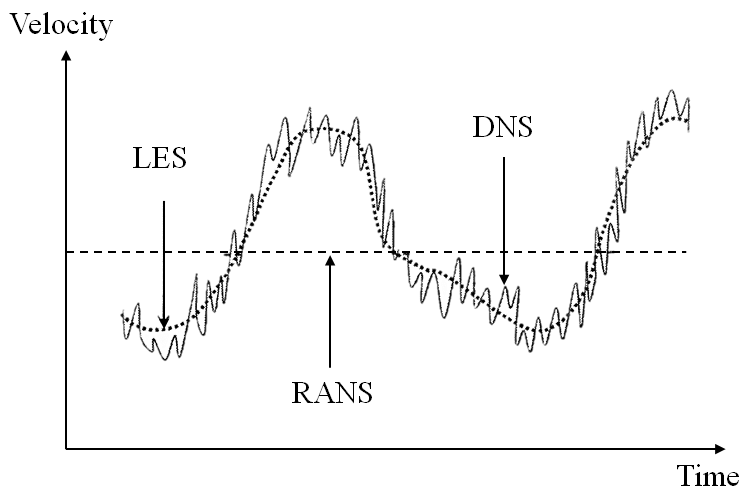
\includegraphics[width=\linewidth]{figures/Literature review/LES.png}
%     \caption{Comparison of turbulence modelling approaches based on their resolution of velocity fluctuations over time. DNS captures all spatial and temporal fluctuations, while LES resolves only the large-scale fluctuations. Adapted from \cite{Foale2021}}    
%   \label{fig: LES}
% \vspace{-1em}
% \end{wrapfigure}


Where $\overline{u}_i$ is the filtered velocity. The filter operation is applied through a filter kernel $G$, where the filter cut-off width is determined to be proportional to the grid size. As seen in \autoref{eq: LESMomentum}, a new term arises $\frac{\partial \tau_{ij}}{\partial x_j}$, which contains the effects of the turbulent scales that the filter operation has cut off. Because most energy is dissipated from a flow in the most minor scales \cite{Turbulence}, this 'Sub Grid Scale' (SGS) tensor needs to be modelled in such a way that it artificially drains enough energy from resolved scales. Many different kinds of SGS models have been proposed, most of which utilise an 'Eddy viscosity' to equate the amount of energy drained to the strain the fluid experiences. The most used eddy viscosity models are ones like the Smagorinsky model (\textcite{Smagorinsky1963}), the  Scale Similarity Model (\textcite{Bardina1980}), the Dynamic Smagorinsky Model (\textcite{Germano1991}, \textcite{Lilly1992}), the Wall-Adapting Local Eddy-viscosity model (\textcite{Nicoud1999}) and the Vreman model (\textcite{Vreman2003}).

\begin{figure}[htb]
  \centering
  % needs: \usetikzlibrary{arrows.meta}  in the preamble
  \definecolor{dnscol}{HTML}{1A1A1A}
  \definecolor{lescol}{HTML}{1F6FB2}
  \resizebox{\textwidth}{!}{%
  \begin{tikzpicture}[>=Stealth, line cap=round, line join=round]
    \def\mean{2.4}
    % ---- RANS / mean line ----
    \draw[red, densely dashed, thick] (0,\mean) -- (15.4,\mean);
    % ---- axes (no tick labels) ----
    \draw[->] (0,0.7) -- (0,4.15) node[above left] {\large $u$};
    \draw[->] (0,0.7) -- (15.9,0.7) node[below] {\large $t$};
    % ---- DNS: resolves all scales (chaotic) ----
    \draw[dnscol, line width=0.4pt] plot coordinates {
    (0.000,3.519) (0.066,3.531) (0.131,3.414) (0.197,3.176) (0.262,3.025) (0.328,3.050)
    (0.393,3.154) (0.459,3.192) (0.524,3.126) (0.590,3.095) (0.655,3.189) (0.721,3.246)
    (0.786,3.207) (0.852,3.154) (0.917,3.186) (0.983,3.300) (1.048,3.341) (1.114,3.254)
    (1.179,3.136) (1.245,2.971) (1.310,2.733) (1.376,2.602) (1.441,2.601) (1.507,2.532)
    (1.572,2.449) (1.638,2.486) (1.703,2.526) (1.769,2.488) (1.834,2.528) (1.900,2.705)
    (1.965,2.813) (2.031,2.748) (2.096,2.699) (2.162,2.764) (2.227,2.804) (2.293,2.779)
    (2.358,2.771) (2.424,2.711) (2.489,2.557) (2.555,2.489) (2.620,2.595) (2.686,2.711)
    (2.751,2.641) (2.817,2.395) (2.882,2.160) (2.948,2.010) (3.013,2.000) (3.079,2.151)
    (3.144,2.315) (3.210,2.463) (3.275,2.652) (3.341,2.760) (3.406,2.737) (3.472,2.647)
    (3.537,2.494) (3.603,2.359) (3.668,2.334) (3.734,2.276) (3.799,2.185) (3.865,2.231)
    (3.930,2.336) (3.996,2.352) (4.061,2.286) (4.127,2.235) (4.192,2.221) (4.258,2.252)
    (4.323,2.357) (4.389,2.455) (4.454,2.496) (4.520,2.531) (4.585,2.567) (4.651,2.519)
    (4.716,2.453) (4.782,2.517) (4.847,2.614) (4.913,2.540) (4.978,2.392) (5.044,2.389)
    (5.109,2.396) (5.175,2.294) (5.240,2.226) (5.306,2.224) (5.371,2.233) (5.437,2.290)
    (5.502,2.242) (5.568,2.024) (5.633,1.870) (5.699,1.921) (5.764,2.164) (5.830,2.377)
    (5.895,2.271) (5.961,1.993) (6.026,1.991) (6.092,2.256) (6.157,2.397) (6.223,2.247)
    (6.288,2.014) (6.354,1.878) (6.419,1.773) (6.485,1.666) (6.550,1.648) (6.616,1.733)
    (6.681,1.782) (6.747,1.711) (6.812,1.566) (6.878,1.487) (6.943,1.575) (7.009,1.667)
    (7.074,1.602) (7.140,1.597) (7.205,1.801) (7.271,1.997) (7.336,1.966) (7.402,1.679)
    (7.467,1.380) (7.533,1.394) (7.598,1.689) (7.664,1.817) (7.729,1.637) (7.795,1.497)
    (7.860,1.486) (7.926,1.447) (7.991,1.408) (8.057,1.447) (8.122,1.554) (8.188,1.642)
    (8.253,1.660) (8.319,1.629) (8.384,1.532) (8.450,1.351) (8.515,1.194) (8.581,1.276)
    (8.646,1.524) (8.712,1.724) (8.777,1.907) (8.843,2.110) (8.908,2.260) (8.974,2.285)
    (9.039,2.162) (9.105,1.929) (9.170,1.719) (9.236,1.629) (9.301,1.639) (9.367,1.729)
    (9.432,1.925) (9.498,2.151) (9.563,2.245) (9.629,2.160) (9.694,2.099) (9.760,2.249)
    (9.825,2.498) (9.891,2.642) (9.956,2.609) (10.022,2.559) (10.087,2.739) (10.153,3.084)
    (10.218,3.346) (10.284,3.447) (10.349,3.337) (10.415,3.119) (10.480,3.061) (10.546,3.157)
    (10.611,3.243) (10.677,3.242) (10.742,3.137) (10.808,2.941) (10.873,2.770) (10.939,2.750)
    (11.004,2.845) (11.070,2.992) (11.135,3.182) (11.201,3.394) (11.266,3.518) (11.332,3.496)
    (11.397,3.383) (11.463,3.229) (11.528,3.090) (11.594,3.029) (11.659,3.066) (11.725,3.158)
    (11.790,3.207) (11.856,3.161) (11.921,3.091) (11.987,3.048) (12.052,2.963) (12.118,2.893)
    (12.183,2.913) (12.249,2.967) (12.314,2.964) (12.380,2.855) (12.445,2.759) (12.511,2.819)
    (12.576,2.898) (12.642,2.785) (12.707,2.603) (12.773,2.563) (12.838,2.680) (12.904,2.812)
    (12.969,2.831) (13.035,2.814) (13.100,2.732) (13.166,2.624) (13.231,2.673) (13.297,2.783)
    (13.362,2.803) (13.428,2.790) (13.493,2.777) (13.559,2.717) (13.624,2.633) (13.690,2.560)
    (13.755,2.491) (13.821,2.439) (13.886,2.413) (13.952,2.361) (14.017,2.399) (14.083,2.620)
    (14.148,2.788) (14.214,2.688) (14.279,2.466) (14.345,2.317) (14.410,2.233) (14.476,2.172)
    (14.541,2.085) (14.607,2.028) (14.672,2.076) (14.738,2.081) (14.803,1.968) (14.869,1.821)
    (14.934,1.735) (15.000,1.712)
    };
    % ---- LES: large scales only (smooth) ----
    \draw[lescol, line width=1.4pt, smooth, tension=0.6] plot coordinates {
    (0.000,3.049) (0.126,3.086) (0.252,3.114) (0.378,3.134) (0.504,3.145) (0.630,3.147)
    (0.756,3.141) (0.882,3.128) (1.008,3.107) (1.134,3.079) (1.261,3.046) (1.387,3.007)
    (1.513,2.964) (1.639,2.918) (1.765,2.869) (1.891,2.819) (2.017,2.769) (2.143,2.718)
    (2.269,2.669) (2.395,2.622) (2.521,2.577) (2.647,2.536) (2.773,2.498) (2.899,2.464)
    (3.025,2.434) (3.151,2.408) (3.277,2.386) (3.403,2.368) (3.529,2.354) (3.655,2.344)
    (3.782,2.336) (3.908,2.330) (4.034,2.326) (4.160,2.324) (4.286,2.321) (4.412,2.319)
    (4.538,2.315) (4.664,2.309) (4.790,2.301) (4.916,2.291) (5.042,2.277) (5.168,2.259)
    (5.294,2.237) (5.420,2.211) (5.546,2.180) (5.672,2.146) (5.798,2.107) (5.924,2.065)
    (6.050,2.019) (6.176,1.971) (6.303,1.921) (6.429,1.869) (6.555,1.817) (6.681,1.765)
    (6.807,1.715) (6.933,1.667) (7.059,1.623) (7.185,1.583) (7.311,1.548) (7.437,1.519)
    (7.563,1.497) (7.689,1.483) (7.815,1.477) (7.941,1.480) (8.067,1.492) (8.193,1.513)
    (8.319,1.543) (8.445,1.583) (8.571,1.631) (8.697,1.689) (8.824,1.754) (8.950,1.826)
    (9.076,1.906) (9.202,1.990) (9.328,2.079) (9.454,2.172) (9.580,2.267) (9.706,2.363)
    (9.832,2.458) (9.958,2.552) (10.084,2.644) (10.210,2.731) (10.336,2.814) (10.462,2.891)
    (10.588,2.960) (10.714,3.023) (10.840,3.076) (10.966,3.121) (11.092,3.157) (11.218,3.183)
    (11.345,3.199) (11.471,3.206) (11.597,3.204) (11.723,3.193) (11.849,3.174) (11.975,3.147)
    (12.101,3.113) (12.227,3.074) (12.353,3.029) (12.479,2.980) (12.605,2.928) (12.731,2.874)
    (12.857,2.820) (12.983,2.765) (13.109,2.711) (13.235,2.659) (13.361,2.610) (13.487,2.564)
    (13.613,2.522) (13.739,2.484) (13.866,2.451) (13.992,2.424) (14.118,2.401) (14.244,2.384)
    (14.370,2.372) (14.496,2.364) (14.622,2.361) (14.748,2.361) (14.874,2.365) (15.000,2.371)
    };
    % ---- legend ----
    \draw[dnscol, line width=0.4pt] (4.6,3.95) -- (5.3,3.95);
    \node[right] at (5.35,3.95) {DNS};
    \draw[lescol, line width=1.4pt] (7.5,3.95) -- (8.2,3.95);
    \node[right] at (8.25,3.95) {LES};
    \draw[red, densely dashed, thick] (10.2,3.95) -- (10.9,3.95);
    \node[right] at (10.95,3.95) {RANS};
  \end{tikzpicture}%
  }
  \caption{Schematic of the velocity signal $u(t)$ at a fixed point as captured by
  the three turbulence-modelling paradigms. DNS resolves the full range of scales;
  LES resolves the large, energy-containing scales and models the sub-filter
  motions; RANS retains only the time-averaged mean.}
  \label{fig: LES}
\end{figure}

Because large-scale structures are directly resolved, LES is more accurate than the RANS approach for the same flow case, as these structures contain most of the turbulent kinetic energy and are responsible for the majority of momentum transfer and mixing. Because LES accuracy depends on the filter width, which in turn is related to the grid spacing, grid refinement will yield more accurate LES results. At the same time, refinement will also significantly increase the computational cost of the simulation. That is why, for high-accuracy flow cases, acceleration frameworks are essential to keep computation costs within usable limits. 

Since the concept of LES was proposed in 1963, it has undergone significant evolution and gained wider acceptance, particularly in academic and research settings. Despite the increase in computational power over the past few decades \cite{Shalf2020}, the cost of performing LES remains higher than that of comparable RANS simulations. This higher cost is due to the need for LES to explicitly resolve the temporal evolution of larger turbulent eddies, which requires finer grid resolutions and more time steps, in contrast to RANS, where the equations are time-averaged and all turbulent fluctuations are modelled.

However, recent academic advancements in LES frameworks, as highlighted by \textcite{Weymouth2025}, suggest that LES can be conducted at relatively low computational cost, even with limited knowledge of the methodology. This perspective aligns with the assertion made by \textcite{Piomelli2014}, who stated that “LES will be used in more complex configurations and will yield reliable results for engineering analysis.”

Despite the high computational cost of LES, advancements in modelling and algorithm design will continue to reduce the cost of high-fidelity simulations. That is why, contrary to \textcite{Zhiyin2015}, we expect LES to be more widely adopted in general engineering applications. Even more so with the acceleration frameworks discussed  \ref{sect: 2.5ML enhancing}.

\section{Machine/Deep learning Enhanced CFD}
\label{sect: 2.5ML enhancing}
The integration of machine learning (ML) into the CFD field offers interesting opportunities to accelerate turbulent flow simulations. While traditional performance-enhancing methods can deliver significant gains, they are constrained by their reliance on numerical algorithms. This is where data-driven methods can complement traditional methods by leveraging the massive amounts of high-fidelity simulation data available. 

% \begin{wrapfigure}{l}{0.5\linewidth}
%     \centering
%     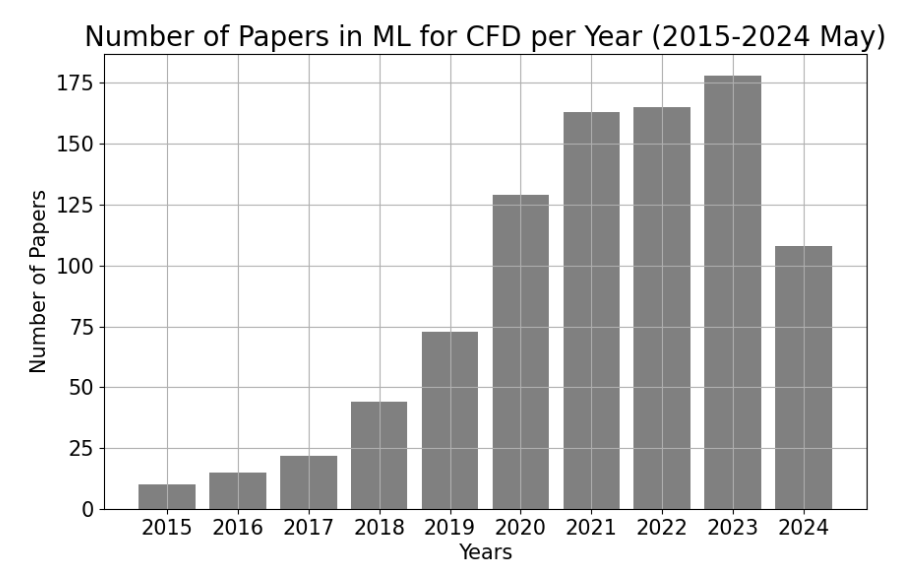
\includegraphics[width=\linewidth]{figures//Literature review/MLpapers.png}
%     \caption{Rise in the amount of ML papers in CFD \cite{Wang2024}}
%     \label{fig: MLPapers}
%     \vspace{-1em}
% \end{wrapfigure}

% \begin{figure}[htpb]
%     \centering
%     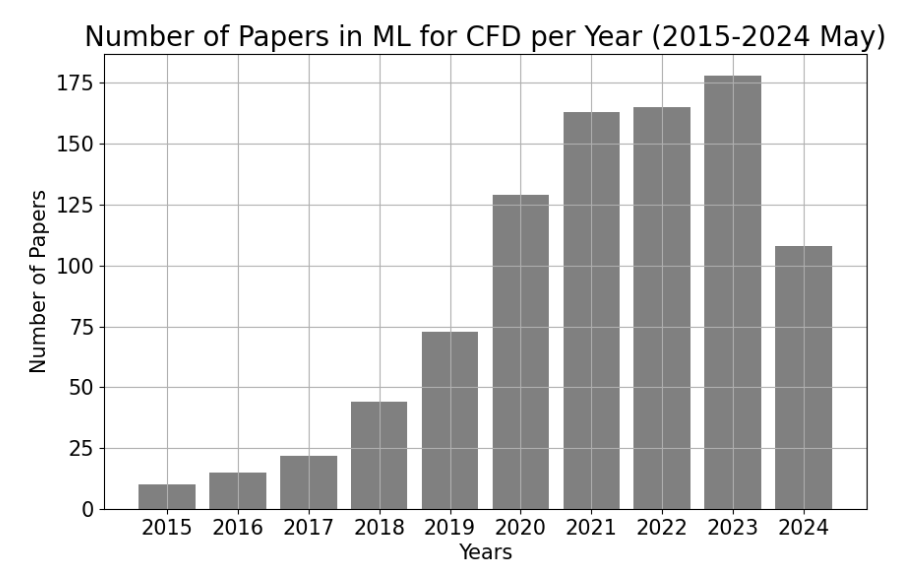
\includegraphics[width=0.5\linewidth]{figures//Literature review/MLpapers.png}
%     \caption{Rise in the amount of ML papers in CFD \cite{Wang2024}}
%     \label{fig: MLPapers}
%     \vspace{-1em}
% \end{figure}



It is worth noting that recent years have seen an exponential growth in the number of studies exploring ML-enhanced CFD. Countless methods incorporating ML into the CFD landscape have been developed, ranging from broadly adopted to more niche applications. Comprehensive reviews, such as those by \textcite{Vinuesa2022} and \textcite{Wang2024}, demonstrate the rapid advancements in the field. Accordingly, this literature review covers relevant ML frameworks that align with the central research question posed in \autoref{chap: Introduction}, prioritising methods aimed at accelerating scale-resolved CFD simulations rather than providing a comprehensive survey of the field. Adjacent applications are therefore only addressed where they directly inform the proposed approach, as it is beyond the scope of this work to cover all relevant contributions in detail.


Before highlighting the current landscape of ML-enhanced CFD simulations, \autoref{subsect: intro to ML} and \autoref{subsect: introtoNN} will briefly handle ML and NN terminology before \autoref{subsect: commonNN} will introduce key neural network architectures which are frequently used in the CFD environment. Where \autoref{subsect: PIsurrogates}, \autoref{subsect: data driven ROMS}, and \ref{subsection: ML solver} will showcase how ML can be leveraged to accelerate CFD simulations by enhancing solver components, employing data-driven ROMS and creating physics-informed surrogate models. 


\subsection{Introduction to Machine Learning}
\label{subsect: intro to ML}
Machine Learning is a branch of artificial intelligence that aims to develop algorithms capable of learning patterns and making predictions from data without being explicitly programmed. ML models can essentially be expressed as a function $\boldsymbol{y}(\boldsymbol{x})$ which takes an input vector $\boldsymbol{x}$ and transforms it to an output vector $\boldsymbol{y}$. The precise form of $\boldsymbol{y}(\boldsymbol{x})$ is determined during the \textit{training phase} based on the training data \cite{bishop2007}. The training of the model requires a dataset that is usually split into training, validation and test sets. The training set is used to fit the model parameters, while the validation set can be used to determine hyperparameters, such as the learning rate and network architecture. The test set evaluates the model's generalisation to unseen data \cite{burkov2020}. 

Depending on the target variable, ML objectives are typically categorised into two categories: regression (continuous outputs such as velocity or pressure predictions) and classifications (discrete categories, e.g., image recognition and Optical Character Recognition).

A central challenge in ML is ensuring that models generalise beyond the training data, meaning that they can reliably generate correct outputs for unseen data that was not in their training set. Overfitting occurs when a model has been trained to achieve an extremely high accuracy on the training data, resulting in poor predictions on unseen test data. While underfitting reflects a model that is too simple to capture the underlying dynamics of the training data, resulting in poor performance even on the training data \cite{burkov2020}. To address these pitfalls, regularisation strategies, careful dataset design, and physically informed constraints can be employed to reduce model complexity and penalise unrealistic predictions \cite{Aggarwal2018, sanderse2024}.

ML algorithms are broadly grouped into three categories: supervised learning, where models learn from labeled data (most common in CFD, like mapping flow fields to forces); unsupervised learning, which identifies patterns or reduced representations from unlabelled data (e.g., clustering coherent flow structures or dimensionality reduction); and reinforcement learning, where an agent interacts with an environment to optimize a reward. 

A detailed treatment of machine learning theory is beyond the scope of this work. Still, it can be found in standard references such as \textcite{bishop2007, burkov2020, danie2021}, which provide the broader theoretical background underlying the CFD-oriented applications discussed further down in this work.

\subsection{Introduction to Neural Networks}
\label{subsect: introtoNN}

% \begin{wrapfigure}{r}{0.5\linewidth}
%     \centering
%     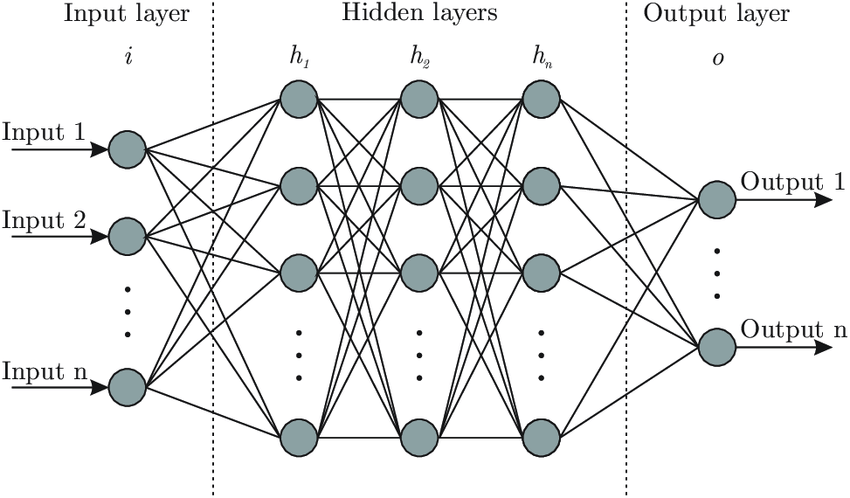
\includegraphics[width=0.8\linewidth]{figures/Literature review/NeuralNetwork.png}
%     \caption{General architecture of a Feed Forward Neural network, adapted from \cite{nashtech_activation2023}}
%     \label{fig: FNN}
% \end{wrapfigure}


Neural networks (NNs) are a class of ML models inspired by the biological nervous system, designed to approximate complex nonlinear functions. They consist of interconnected computational units, or neurons, which receive inputs, process them through an activation function and produce an output. A general architecture of a NN can be seen in \autoref{fig: FNN}. The use of non-linear activation functions enables NNs to act as universal function approximators \cite{Hornik1989}, capable of representing highly complex mappings between inputs and outputs. 

\begin{figure}[htb]
    \centering
    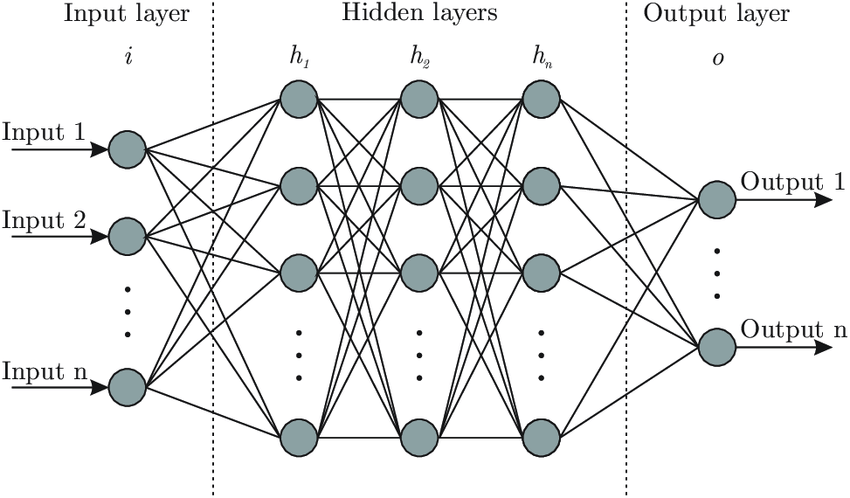
\includegraphics[width=0.85\linewidth]{figures/Literature review/NeuralNetwork.png}
    \caption{General architecture of a Feed Forward Neural network, adapted from \cite{nashtech_activation2023}}
    \label{fig: FNN}
\end{figure}


Training a neural network involves minimising a loss function that quantifies the difference between predictions and actual values across the dataset. This optimisation is typically performed via gradient descent and its variants, with gradients computed efficiently using backpropagation \cite{Aggarwal2018}. To achieve a desirable accuracy, hyperparameters such as learning rate, network depth, and activation function can be optimised by monitoring the network's performance. After training is completed, a set of weights and biases is created that defines how the network transforms inputs into outputs.

The architecture of an NN can significantly affect its performance on different tasks. The simplest form of NNs are feed-forward neural networks (FNNs), as seen in \ref{fig: FNN}, where information flows from input to output in a single pass.

% where the NN displays an input layer on the left, hidden layers in the middle and an output layer on the right. A network where information flows follows this path is called a feed-forward neural network (FNN) \cite{Aggarwal2018}.

\subsection{Common Neural Network Architectures Employed in CFD}
\label{subsect: commonNN}

\subsubsection{Convolutional Neural Networks}
Convolutional Neural Networks (CNNs) are a frequently used class of neural networks specifically designed to process grid-structured input data that exhibit strong spatial dependencies in local regions of the grid \cite{Aggarwal2018}. That is why CNNs are often used for image recognition, since adjacent spatial locations in an image often have similar pixel colour values. CNNs are characterised by convolution operations, which involve taking a dot product between a grid-structured set of weights (known as a filter or kernel) and the input data to extract features.

Because of the strong capabilities of CNNs to extract features from image snapshots, they present themselves as good candidates to be implemented for CFD predictions. Since CFD flow fields can be represented as a structured grid, CNNs offer an outstanding possibility to learn patterns such as vortices or boundary layers effectively. This can be helpful for tasks such as flow prediction, surrogate modelling, or acceleration \cite{Lee_You_2019, Guo2016}.

\todo{Add figure of convolutional NN}

% \subsubsection{Recurrent Neural Networks}

% Recurrent Neural Networks (RRNs) are specifically designed for sequential data, where elements are ordered and depend on the value of the previous component of the series. Unlike traditional FFNs, RNNs take the inherent order of the data into account by processing inputs in sequence and treating them similarly relative to previous inputs. This behaviour is achieved by sharing the same set of network parameters across different temporal layers, allowing the network to maintain a hidden state that changes with each new input, effectively acting as a memory of past information \cite{Aggarwal2018}. 

% However, RNNs often struggle to predict long-term dependencies due to the vanishing and exploding gradient problem, which can arise during training. To address this, a variant of RNNs called Long Short-Term Memory (LSTM) networks uses internal memory and gating mechanisms to regulate how information is stored, updated, or forgotten, enabling them to manage long-term dependencies more effectively. An overall structure of an LSTM is displayed in \autoref{fig: LSTM}, showing how the internal memory state $c_t$ refers to the work by \textcite{Aggarwal2018}, which provides an in-depth theoretical analysis of LSTMs, which are considered to be outside the scope of this literature review. For a more detailed explanation of RNNs, LSTMs, and the vanishing and exploding gradient problem, please refer to the work by \textcite{Aggarwal2018}, which provides an in-depth theoretical analysis of these concepts. 

% \begin{figure}[h]
%     \centering
%     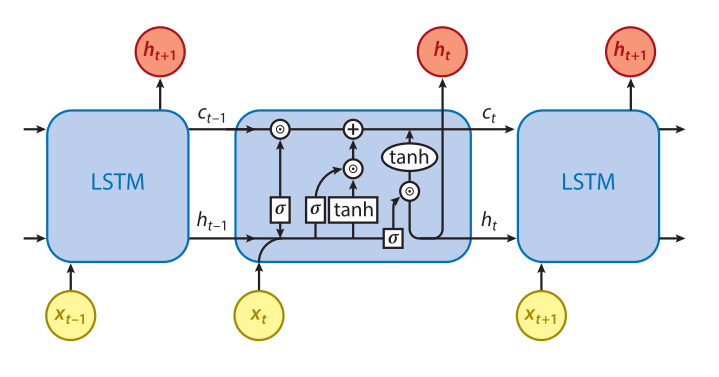
\includegraphics[width=0.75\linewidth]{figures//Literature review/LSTM.png}
%     \caption{Structure of an LSTM cell with input, forget, and output gates regulating information flow through the memory cell. Source \cite{Brunton2020}}
%     \label{fig: LSTM}
% \end{figure}

% LSTMs are particularly useful in CFD because fluid dynamics is inherently a transient environment, where time-dependent phenomena play a key role in accurate simulations. LSTMs generally excel at predicting temporal sequences and capturing complex non-linear dynamics over longer durations \cite{Aggarwal2018}. These capabilities have been demonstrated to enhance CFD simulations and will be showcased later in this work. 


\subsubsection{Neural Ordinary Differential Equations}
\label{subsubsect: NODEs}

Neural Ordinary Differential Equations (NODEs) are a type of deep neural network model introduced by \textcite{Chen2018} that differ substantially from conventional neural networks. They are similar to RNNs \todo{mention that the discrete analogous model for NODEs are RNN}, and more specifically, Residual Neural Networks (ResNETs \cite{He2015}). In a ResNet, the latent space is represented by a stack of layers, as shown in \autoref{fig: ResNet}. NODEs learn the mapping from sequential data by using a continuous representation of the latent space. 




\begin{figure}[htp]
    \centering
    % 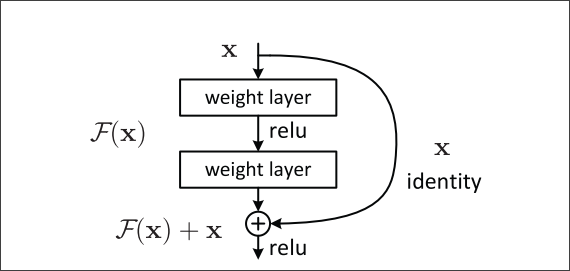
\includegraphics[width=0.6\linewidth]{figures/Literature review/swappy-20260616-174354.png}
    
  \begin{tikzpicture}[
      box/.style={draw, minimum width=2.6cm, minimum height=0.6cm, font=\small},
      >=latex,
      node distance=0.9cm
    ]
    % --- main column ---
    \node (x) {$\mathbf{x}$};
    \node[box, below=0.55cm of x] (w1) {weight layer};
    \node[box, below=0.9cm of w1] (w2) {weight layer};
    \node[circle, draw, inner sep=1.6pt, below=0.55cm of w2] (plus) {$+$};

    % branch point on the line between x and w1
    \coordinate (branch) at ($(x)!0.55!(w1)$);

    % --- main path arrows ---
    \draw[->] (x) -- (w1);
    \draw[->] (w1) -- (w2) node[midway, right] {relu};
    \draw[->] (w2) -- (plus);
    \draw[->] (plus) -- ++(0,-0.85) node[midway, right] {relu};

    % --- identity / skip connection (curves right then into +) ---
    \draw[->] (branch) -- ++(2.00,0) |- (plus);

    % --- side labels ---
    \node[left=0.35cm of w1, font=\normalsize] {$\mathcal{F}(\mathbf{x})$};
    \node[left=0.35cm of plus, font=\normalsize, anchor=east, xshift=-0.1cm]
      {$\mathcal{F}(\mathbf{x})+\mathbf{x}$};
    \node[right=1.00cm of w2, align=left] {$\mathbf{x}$\\identity};
  \end{tikzpicture}

    \caption{ResNet layer stacking, adapted from \cite{He2015}}
    \label{fig: ResNet}
\end{figure}


% \begin{figure}[htbp]
%     \centering
%     \begin{subfigure}[t]{0.48\textwidth}
%         \centering
%         
  \begin{tikzpicture}[
      box/.style={draw, minimum width=2.6cm, minimum height=0.6cm, font=\small},
      >=latex,
      node distance=0.9cm
    ]
    % --- main column ---
    \node (x) {$\mathbf{x}$};
    \node[box, below=0.55cm of x] (w1) {weight layer};
    \node[box, below=0.9cm of w1] (w2) {weight layer};
    \node[circle, draw, inner sep=1.6pt, below=0.55cm of w2] (plus) {$+$};

    % branch point on the line between x and w1
    \coordinate (branch) at ($(x)!0.55!(w1)$);

    % --- main path arrows ---
    \draw[->] (x) -- (w1);
    \draw[->] (w1) -- (w2) node[midway, right] {relu};
    \draw[->] (w2) -- (plus);
    \draw[->] (plus) -- ++(0,-0.85) node[midway, right] {relu};

    % --- identity / skip connection (curves right then into +) ---
    \draw[->] (branch) -- ++(2.00,0) |- (plus);

    % --- side labels ---
    \node[left=0.35cm of w1, font=\normalsize] {$\mathcal{F}(\mathbf{x})$};
    \node[left=0.35cm of plus, font=\normalsize, anchor=east, xshift=-0.1cm]
      {$\mathcal{F}(\mathbf{x})+\mathbf{x}$};
    \node[right=1.00cm of w2, align=left] {$\mathbf{x}$\\identity};
  \end{tikzpicture}

%     \caption{ResNet layer stacking, adapted from \cite{He2015}}
%     \label{fig: ResNet}
%     \end{subfigure}
%     % \hfill
%     \begin{subfigure}[t]{0.48\textwidth}
%         \centering
%      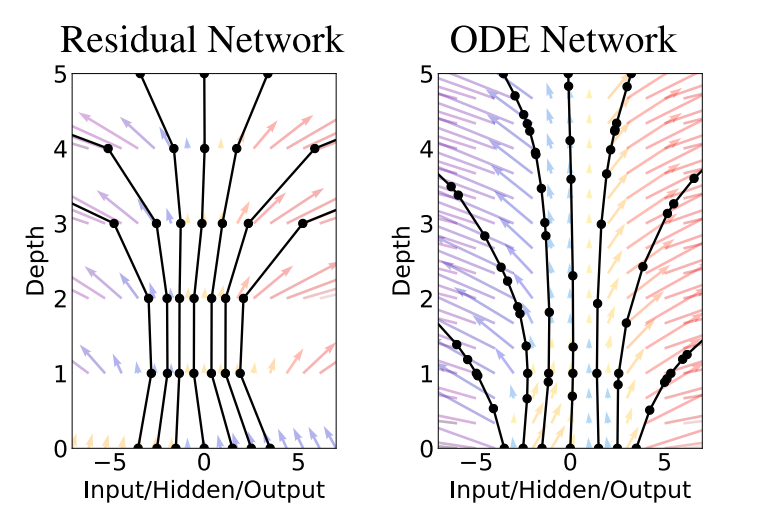
\includegraphics[width=\linewidth]{figures//Literature review/latentspace.png}
%     \caption{Left: Discrete evolution of ResNet predictions, Right: continuous evolution of predictions by NODE. Adapted from \cite{Chen2018}}
%     \label{fig: latentspace}
%     \end{subfigure}
%     \caption{general caption}
% \end{figure}
% \begin{wrapfigure}{r}{0.45\textwidth}
% \vspace{-1em}
%     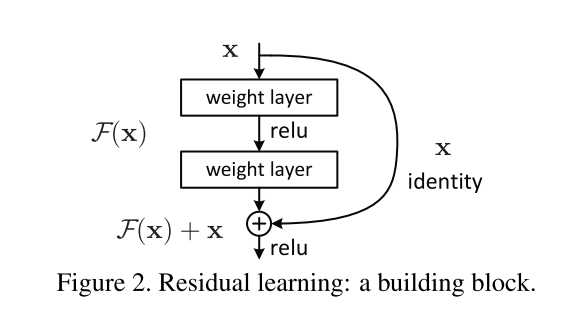
\includegraphics[width=1\linewidth]{figures//Literature review/ResNet.png}
%     \caption{ResNet layer stacking, adapted from \cite{He2015}}
%     \label{fig: ResNet}
% % \vspace{-1em}
% \end{wrapfigure}

Where the stacking of the latent state in ResNets can be seen as an Euler discretisation of a continuous transformation, shown in \autoref{eq: euler}

\begin{equation}\label{eq: euler}
    h_{t+1} = h_t + f(h_t, \theta_t)
\end{equation}

Where $h_{t+1}$ is the newly determined latent state, which is constructed of a summation of the current latent state $h_t$ through the addition of a function of the network parameters $\theta_t$ and the value of the current prediction $f(h_t, \theta_t)$, when the added layers become large and the steps taken become smaller, this progression of the latent state can be represented by a differential equation \ref{eq: NODeODE}. 

\begin{equation}\label{eq: NODeODE}
   dh(t)/dt = f(h(t), t, \theta) 
\end{equation}

A conventional ODE solver can then be used to solve this equation. This formulation provides adaptive computation capabilities, as ODE solvers can dynamically adjust step sizes based on the solution's complexity, enabling an optimal trade-off between speed and accuracy. This essentially allows NODEs to define a smooth flow through the latent space, rather than the discrete series of transformations that ResNets produce. \autoref{fig: latentspace} shows a graphical representation of the latent space vector field.

\begin{figure}
    \centering
   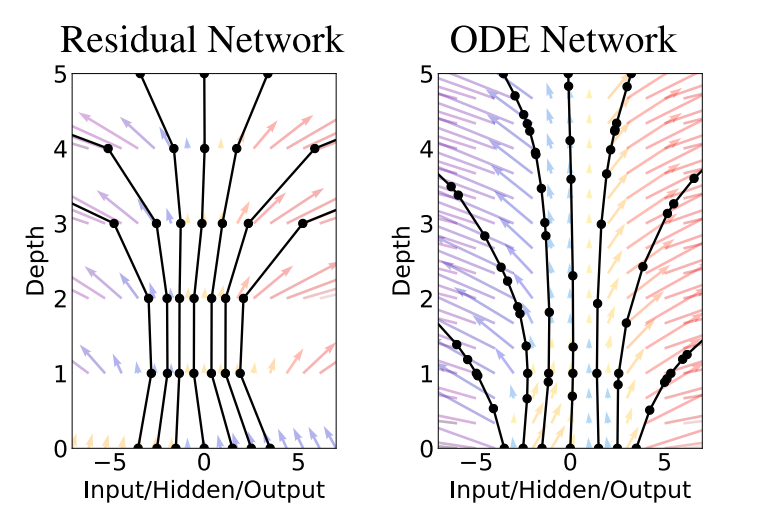
\includegraphics[width=.55\linewidth]{figures//Literature review/latentspace.png}
    \caption{Left: Discrete evolution of ResNet predictions, Right: continuous evolution of predictions by NODE. Adapted from \cite{Chen2018}}
    \label{fig: latentspace}
\end{figure}

% \begin{wrapfigure}{r}{0.45\textwidth}
%     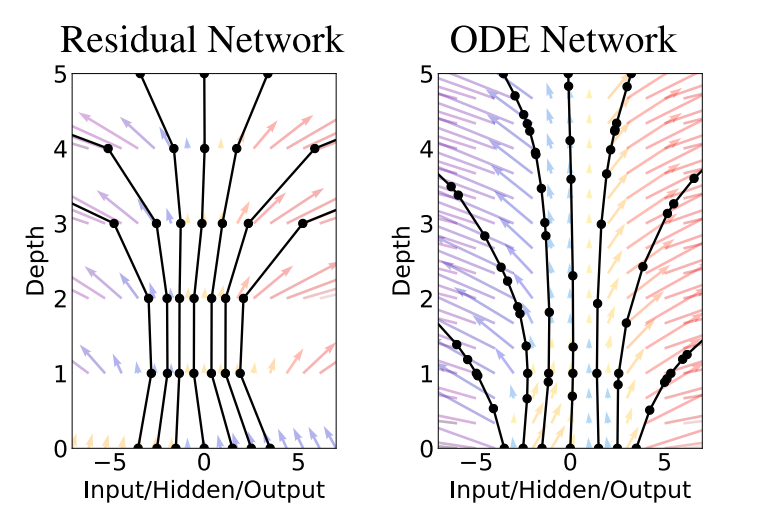
\includegraphics[width=1\linewidth]{figures//Literature review/latentspace.png}
%     \caption{Left: Discrete evolution of ResNet predictions, Right: continuous evolution of predictions by NODE. Adapted from \cite{Chen2018}}
%     \label{fig: latentspace}
% \end{wrapfigure}

NODEs also provide a memory-efficient way to train deep models using the adjoint sensitivity method, which propagates through the ODE by solving a second augmented ODE backwards in time. Because the neural network can be viewed as a universal approximator, and the ODE solver can evaluate the latent layers at any time point and timestep, the resulting model provides smooth predictions without being constrained to discrete time steps or layers. This behaviour makes NODEs particularly well-suited for predicting systems where continuous-time behaviour is essential, even when the supplied training data is irregularly sampled in time. 

In the context of CFD time-series prediction, NODEs can offer key advantages. Their adaptive behaviour can enable variable-time-step integration, which can be optimal for accelerating potential CFD simulations. However, since NODEs involve solving ODEs and fluid systems are often high-dimensional, solving these ODEs can be computationally intensive. That is why, in recent literature, such as the work of \textcite{Shankar2022}, NODEs have been implemented within data-driven reduced-order models, where the dynamics of the latent space are predicted using NODEs. This aligns with the objective of this thesis, where instead of predicting the time integration of the NSE, the authors have implemented NODEs in the latent space of a ROM, which is used to predict the entirety of the latent dynamics, which can then be used as a surrogate model for a specific flow case. 

Another recent advancement in Neural ODE research has been the implementation of a physics-informed loss term. This embeds the governing equations of the system that the model aims to predict directly into the training process. \textcite{Sholokhov2023} introduced a collocation-based physics-informed loss function that enforces PDE constraints at sampled points, improving extrapolation, stability, and performance in situations where there is not a lot of training data available. Additionally, \textcite{Ghanem2025} proposed an optimisation framework that incorporates physics-informed loss terms, enabling the accurate recovery of hidden states when only partial measurements are available as training data. These works demonstrate that embedding physical laws into the NODE loss function allows for a more robust model in scenarios with sparse, noisy, or incomplete data. This approach could be particularly valuable in CFD, where enforcing conservation laws and physical consistency can lead to better flow-field predictions with fewer training data. 

 
\subsection{Machine Learning Enhanced Solver Components}
\label{subsection: ML solver}

One way to leverage ML to accelerate scale-resolved CFD simulations is to embed machine learning directly into specific components of CFD solvers. Rather than learning the whole flow evolution, these approaches aim to improve the efficiency and accuracy of key solver stages. Calculations such as the Pressure-Poisson equation, RANS turbulence closure models, sub-grid scale models, or even learning-based discretisation are all possibilities that have been presented in recent literature. 

\subsubsection{Pressure-Poisson prediction}
As mentioned previously, an essential component of incompressible CFD solvers is the pressure-velocity coupling algorithm, which ensures that the computed velocity field remains divergence-free. This coupling is typically enforced in operator splitting methods to discretise the NSE, where first the velocity field is advected, and the resulting velocity field $\mathbf{u^*}$ does not satisfy the continuity equation \ref{eq: continuity}. This is then corrected using the Pressure-Poisson Equation (PPE) \ref{eq: PPE} \cite{Vinuesa2022}. 

\begin{equation}\label{eq: PPE}
    \frac{\Delta t}{\rho} \nabla^2 p = -\nabla \cdot \mathbf{u}^*
\end{equation}

Where $\Delta t$ is the simulation time step, $\rho$ the fluid density and $p$ the pressure field, finding the solution to this equation is typically the most computationally expensive for the numerical solver. This is why exploring alternative strategies for this computation could yield promising acceleration. 

\textcite{Chen2022} proposed a framework which employed a multi-scale Graph Neural Network (GNN) to either entirely or partially replace the traditional iterative PPE solver. Using this framework, the authors achieved solution speeds nearly three times faster for a Reynolds number of 1000 and almost twice as fast for 5000 in the training datasets. Additionally, \textcite{Ajuria2020} developed a hybrid computational strategy to accelerate the PPE computation. The authors propose a method using Convolutional Neural Networks (CNNs) to predict the pressure field in addition to the traditional Jacobi solver. Using this hybrid method, the authors achieved significant speed-ups of up to 320\% while maintaining the predetermined accuracy. The authors, however, do not mention how long it took to generate the training data and how long the CNN training took. 

Recently, \textcite{Sousa2024} proposed a versatile ML-based method applicable to various geometries. The developed ML models utilise Multilayer Perceptron (MLP) neural networks combined with Principal Component Analysis (PCA) transformations. This combination has proven to be efficient and trainable, requiring relatively low computational resources, and achieves acceptable accuracy with errors of around 3\%. However, the authors note that the surrogate models struggle with extrapolating into significantly different flow regimes. To address this limitation, they suggest diversifying the dataset to enhance the models' practical applications.

\subsubsection{Turbulence modelling}
In the context of RANS simulations, the modelling of the RST is essential for providing closure to the Reynolds-averaged simulation \ref{eq: RANS}. Traditional closure models, such as eddy viscosity models, often rely on empirical formulations which may not generalise well across different flow conditions. To address these limitations, ML frameworks are being proposed to offer a promising approach for developing data-driven turbulence models that can learn more accurate and applicable representations of the RST from high-fidelity data (like DNS or experimental results). 

One of the most notable models is the one by \textcite{Ling2016}, which leverages a custom-built Deep NN architecture which forces the network to make physically accurate predictions. This was achieved by embedding Galilean invariance into the predicted tensor, which improved the network's performance, enabling it to outperform traditional eddy viscosity models \cite{Vinuesa2022}. More recently, \textcite{Cai2024} proposed an improved version of the Tensor Basis Neural Network (TBNN), which builds upon the work of \textcite{Ling2016}. Their proposed framework used MLPs and a loss function which employed a weighted MSE based on the Reynolds stress anisotropy tensor components. Using this approach, they achieved a global R$^2$ improvement from approximately 0.7 to 0.9982 for Square Duct Flow (SDF). They significantly improved the prediction of the components of the Reynolds stress anisotropy tensors from 0.3295 to 0.9899 for specific entries. Furthermore, transfer learning was also implemented to circumvent data scarcity, which improved performance and delivered faster convergence with only 10\% of the training data.

Although recent models, such as the aTBNN \cite{Cai2024}, and more recent works, like \cite{Girimaji2024, Jiang2021, Sanhueza2023}, have shown clear improvements over conventional models, ML-based turbulence modelling is still not ready for widespread use in engineering practice. The models often work well on the flows they are trained on, but struggle to generalise to new or complex cases. Recently, the NASA Symposium on Turbulence Modelling \cite{Rumsey2022}, along with a self-released paper by Spalart \cite{Spalart}, highlighted that there are still fundamental issues in the RANS framework, and machine learning alone will not resolve them. The limited (but increasing) amount of high-fidelity data available, combined with the lack of robustness in industrial settings, makes it challenging for engineers to trust these models fully. As a result, despite the interesting progress, the field still faces growing pains and will need collective transparency and standardisation before it can be used reliably in real-world applications. 


\subsubsection{Sub grid scale modelling}
Similar to the closure problem in RANS modelling, LES needs to model the effect of the sub-grid scales on the resolved scales to ensure accurate simulations. Conventional SGS models typically rely on case-specific constants, such as scale similarity \cite{Bardina1980} or eddy viscosity \cite{Lilly1992, Germano1991}, which may not be applicable across all flow regimes and can lead to significant errors if not correctly configured. With the increasing availability of high-fidelity data and improved computational resources \cite{ansys2023multiGPU, Chen2009}, ML can offer alternative SGS models that are more adaptive, providing the potential to capture the complex interactions between turbulent scales. 

\begin{wrapfigure}{r}{0.45\textwidth}
    \centering
    % 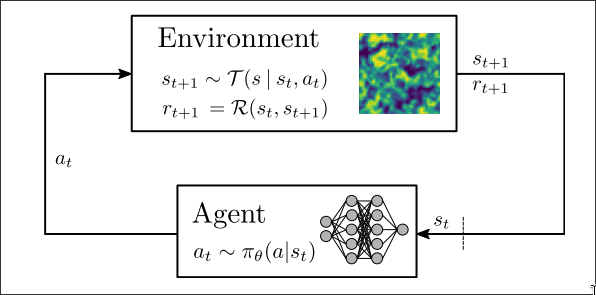
\includegraphics[width=\linewidth]{figures//Literature review/RL_LES.png}
    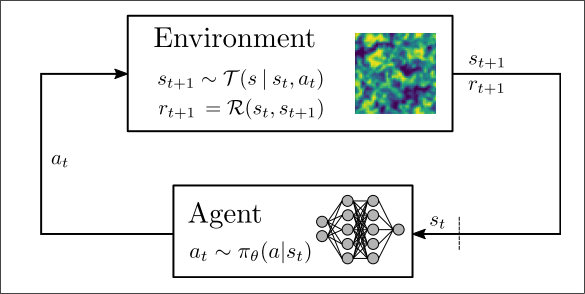
\includegraphics[width=\linewidth]{figures//Literature review/swappy-20250830-000913.png}
    \caption{The agent interacts with the LES environment to adapt the eddy viscosity dynamically based on the local flow state, adapted from \cite{Kurz2023}}
    \label{fig: RLSGS}
\end{wrapfigure}

ML has been used to develop SGS models in basically two ways: supplementing the unresolved energy in the coarse mesh using supervised learning and developing reinforcement learning approaches to stabilise the coarse simulation \cite{Vinuesa2022}. For the first approach, numerous studies exist that employ high-fidelity data to train deep learning models. The goal is to train these models to map the energy of the small-scale structures of the fine grid DNS data to the coarse LES mesh. The first one to propose such a model was \textcite{Beck2019}, who employed CNNs to determine the underlying unknown non-linear mapping from the coarse grid quantities to the closure terms without a priori assumptions \cite{Beck2019}. They achieved a cross-correlation of 47\% in decaying homogeneous isotropic turbulence. Alternatively, \textcite{Sirignano2023} developed ML closure models for LES of incompressible flows around bluff bodies.  Unlike a priori methods that train neural networks before implementing them into the CFD solver, they proposed an a posteriori approach, which directly optimises the neural network parameters by solving the LES equations and their adjoints. Their ML-LES models significantly outperformed commonly used dynamic Smagorinsky and Anisotropic Minimum-Dissipation (AMD) \cite{Rozema2015} models in a posteriori predictions, even on relatively coarse meshes. Even when training the model on rectangular bluff bodies, their framework showed promising results for out-of-sample bluff body shapes. This indicates that ML frameworks for LES closure models can be generalised to alternative flow cases if their architecture and training samples are adapted accordingly. 


An example of reinforcement learning being employed for developing a data-driven SGS model is the work by \textcite{Kurz2023}. This method addresses the inconsistency of supervised learning for implicitly filtered LES, where the exact form of the implicit filter is typically unknown, making it impossible to compute corresponding closure terms a priori. By formulating turbulence modelling as an RL task, the agent, based on a CNN-based policy, interacts directly with the dynamical LES environment to dynamically adapt the eddy viscosity in space and time, based solely on the local flow state. Starting from an initial flow state, the agent will keep interacting with the environment until a desirable state is reached, an overview of this process is shown in \autoref{fig: RLSGS}. The research demonstrates that the trained RL-based models achieve long-term stable simulations and significantly outperform established analytical models in accuracy, while also exhibiting strong generalizability to different resolutions and higher Reynolds numbers not seen during training.

The examples highlighted are just a few of many ML-SGS models proposed; the work by \textcite{Vinuesa2022} offers a more detailed overview of alternative proposals for the same closure problem. However, similar to the RANS closure problem, these ML-SGS still suffer from poor generalizability. This is mainly due to the limited DNS data, which is often only available at low Reynolds numbers \cite{sanderse2024}. 

\subsection{Data-Driven Reduced Order Models}
\label{subsect: data driven ROMS}
 Data-driven reduced-order models have been utilised to accelerate CFD simulations by approximating high-fidelity systems in a lower-dimensional form that retains most of the relevant flow phenomena. Data-driven ROMs extract dominant patterns from simulation or experimental snapshots without requiring explicit knowledge of the appropriate governing equations. Unlike physics-based ROMs, which typically use linear projections (such as POD) to solve the NSE on a basis with a reduced number of DOFs, data-driven ROMs rely on snapshots of the full-dimensional state vector to produce projection operations through a training process. This utilises the previously explained capabilities of neural networks to approximate a nonlinear function. These methods can achieve significant speedups after being successfully trained on supplied CFD snapshot data, or they can be used in a transfer learning fashion to accelerate CFD simulations, as will be explained in further detail. 

\begin{figure}[h]
    \centering
    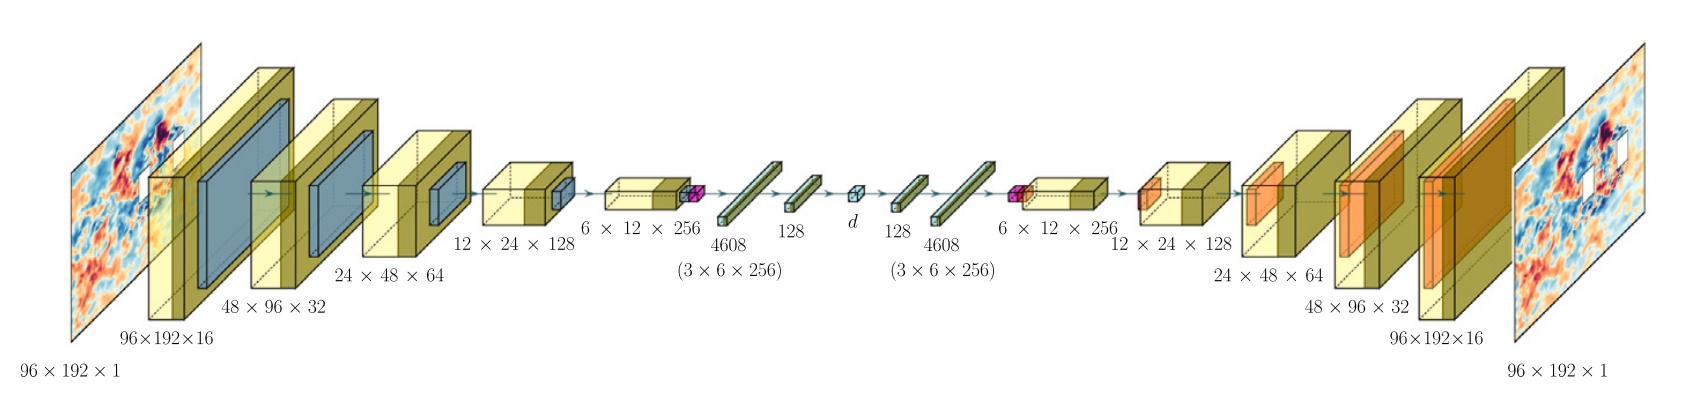
\includegraphics[width=1\linewidth]{figures//Literature review/CNN-Autoencode.png}
    \caption{Schematic view of a CNN autoencoder extracting non-linear modes from a CFD snapshot, source \cite{Eivazi2022}}
    \label{fig: CNN encoder}
\end{figure}

Data-driven ROMs employ the same working principles as autoencoders, specifically the use of the encoder and decoder network architectures. The encoder compresses the high-dimensional snapshots into a lower-dimensional latent space, and the decoder reconstructs this latent space back to the exact dimensions as the input snapshots, while minimising reconstruction error. The usage of non-linear activation functions within the autoencoder allows the network to capture the complex non-linear behaviour of turbulent structures. This offers a key advantage over methods like POD, which are limited to linear representations \cite{Pant2021}. For processing spatial data of fluid flows, autoencoders often integrate CNNs into their architecture due to their good results with grid-structured data. \autoref{fig: CNN encoder} shows an overview of how an autoencoder reduces and reconstructs a single CFD snapshot to and from a latent space. 

% \todo{rewrite these paragraphs}
What differs data-driven ROMs from autoencoders is the requirement that the latent space must also capture and predict the temporal dynamics of the system. This means that, in addition to learning a compact representation of the input data, the latent variables must be predicted in a way that accurately reproduces the future state of the simulation \cite{Vinuesa2022}. This can be achieved by either selecting the dimensions of the latent space in a way that allows for a correct prediction of the future flow field, or by utilising regression architectures that are better suited for time series prediction, such as RNNs, LSTMs, or neural ODEs. 

\begin{figure}[h]
    \centering
    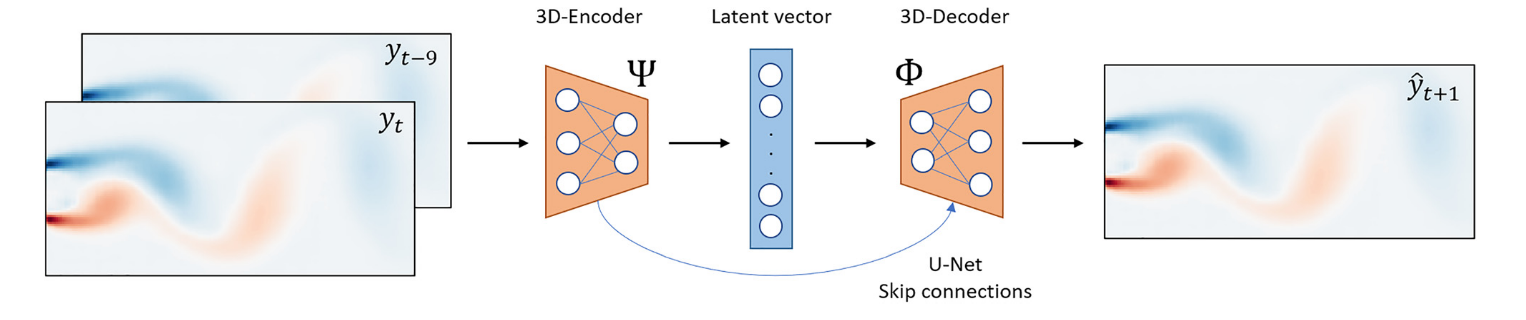
\includegraphics[width=1\linewidth]{figures//Literature review/DL-ROM.png}
    \caption{Example architecture of deep convolutional ROM, source \cite{Pant2021}}
    \label{fig: DL-ROM}
\end{figure}

Some notable examples of deep learning-based ROMs include the work of \textcite{Pant2021}, where the authors leveraged 3D Autoencoder and 3D U-Net-based architectures to create non-linear projections from reduced-order states to fluid flow snapshots, as depicted in \autoref{fig: DL-ROM}. The authors employ a looped prediction strategy, where the last 10 snapshots of a simulation are used to train the network to predict the following timestep $\hat{y}_{t+1}$. This prediction is then appended to the last nine snapshots and used as input to predict $\hat{y}_{t+2}$. This process is repeated recursively for 20 timesteps. This looping strategy allowed a reduction in simulation speed of 2 orders of magnitude \cite{Pant2021}. Similarly, CFDnet \cite{Obiols-Sales2020} accelerates RANS simulations by leveraging its CNN ROM to predict fluid properties, while still utilising the CFD solver to ensure that domain-specific convergence constraints are met. This allowed the authors to deliver highly accurate predictions while still achieving acceleration rates from 1.9 up to 7.7 times the benchmark simulations. 

\begin{wrapfigure}{r}{0.45\textwidth}
    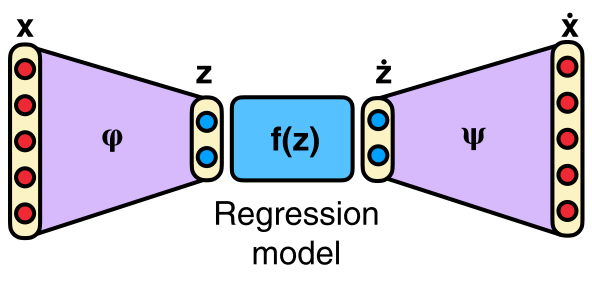
\includegraphics[width=\linewidth]{figures//Literature review/DL-regression-ROM.png}
    \caption{Example architecture of autoencoder with regression in the latent space, adapted from \cite{Vinuesa2022}}
    \label{fig: ROM regressor}
\end{wrapfigure}

As previously mentioned, the dynamics in the latent space can also be modelled by utilising a regressor in the latent space of the autoencoder, which would make the architecture of the data-driven ROM look like \autoref{fig: ROM regressor}. A notable example of such an architecture is the work by \textcite{Shankar2022}, which demonstrates how NODEs are utilised to model system dynamics in the latent space. By explicitly decoupling the reduction and latent system dynamics, the presented framework achieved very accurate reconstructions of flow dynamics over large integral timescales. Instead of using NODEs for the dynamical modelling in the latent space, LSTMs can also be used, as they present good capabilities for time series predictions, as indicated in the work by \textcite{Mohan2019}.

\subsection{Physics Informed Surrogate Models}
\label{subsect: PIsurrogates}
Physics-informed surrogate models demonstrate strong potential in accelerating computationally intensive simulations. A surrogate model is a broad term for a computationally efficient approximation of a complex system. A ROM, which was handled previously, is a specific type of surrogate that reduces the system's dimensionality by applying a projection to the high-dimensional dynamics in a lower-dimensional space. Meaning that all ROMS are essentially surrogate models, not all surrogates are ROMS. 

Where purely data-driven surrogate models, such as DeepONet \cite{Lu2021}, require a large amount of data for reliable prediction performance. In real-world scenarios, where data is either sparse or prohibitively expensive to collect, models that can generalise effectively on smaller datasets are necessary \cite{Donnelly2024}. That is why physics-informed surrogate models embed fundamental physical laws and constraints directly into their architecture or training process. This integration aims to create efficient approximations that are not only accurate but also physically consistent, even when dealing with limited training data \cite{Raissi2019}. 

The integration of physics into these models is achieved mainly through two key mechanisms: physics-informed loss functions and specialised network architecture. Physics-informed loss functions incorporate the residuals of the governing partial differential equations, such as conservation of mass \ref{eq: continuity} and momentum \ref{eq: momentum}, into the loss function during training. This way, the model can be regularised during training, showing bigger errors for predictions which violate the relevant physical laws. Essentially, an artificial bias is added to the network, which promotes data efficiency since the projections are inherently directed to adhere to physical laws. \autoref{eq: physicsloss} shows a general form of a physics-informed loss function, where $\mathcal{L}_{\text{data}}$ is a standard loss function like MSE or MAE, and $\mathcal{L}_{\text{physics}}$ can be derived from the physical system the network has to learn. In the case of a CFD simulation, this latter part can be built from the continuity and momentum equations. These two loss functions can then be combined using a weighted sum, with $\lambda_d$ and $\lambda_p$ serving as weights.

\begin{equation}\label{eq: physicsloss}
\mathcal{L} = \lambda_d \, \mathcal{L}_{\text{data}} 
+ \lambda_p \, \mathcal{L}_{\text{physics}} 
\end{equation}

A prominent example is Physics Informed Neural Networks (PINNs), first proposed by \textcite{Raissi2019}, that use deep learning to solve PDEs, exploiting the concept of automatic differentiation used in the back propagation algorithm to calculate partial derivatives \cite{Vinuesa2022}. PINNs have been utilised in various CFD scenarios, including hydrodynamic surrogate models \cite{Donnelly2024}, high-speed flow approximations \cite{Mao2020}, and more general NS cases \cite{Eivazi2021, Sun2019}, where they have demonstrated excellent results in predicting flow parameters with limited training data. However, in the context of accelerating fluid simulations, PINNs have a disadvantage in that their training speed restricts them from achieving significant speed-up results in a CFD workflow \cite{Jeon2024, Go2023}. On the other hand, PINNs have been successfully used as closure models for RANS and LES frameworks; the workings of this will be explained later in this literature review. 

Alternatively to PINNs, the Finite Volume Method Network FVMN \cite{Jeon2022} is a physics-informed surrogate model which specifically exemplifies a physics-informed surrogate model tailored for CFD, integrating principles of the finite volume method (FVM) directly into its design. Unlike previously explained methods that only include information about a single grid point, FVMN employs a tiered input system that incorporates physical quantities from a central grid point and its neighbouring grid points into the input matrix of the neural network. This allows the network to imitate the mass and heat transport among neighbouring cells, which is considered the most crucial process in the FVMN. Additionally, instead of directly predicting the future state, FVMN employs a derivative output system, which means it predicts the change or derivative of physical quantities over a given time step. 

\begin{figure}[h]
    \centering
    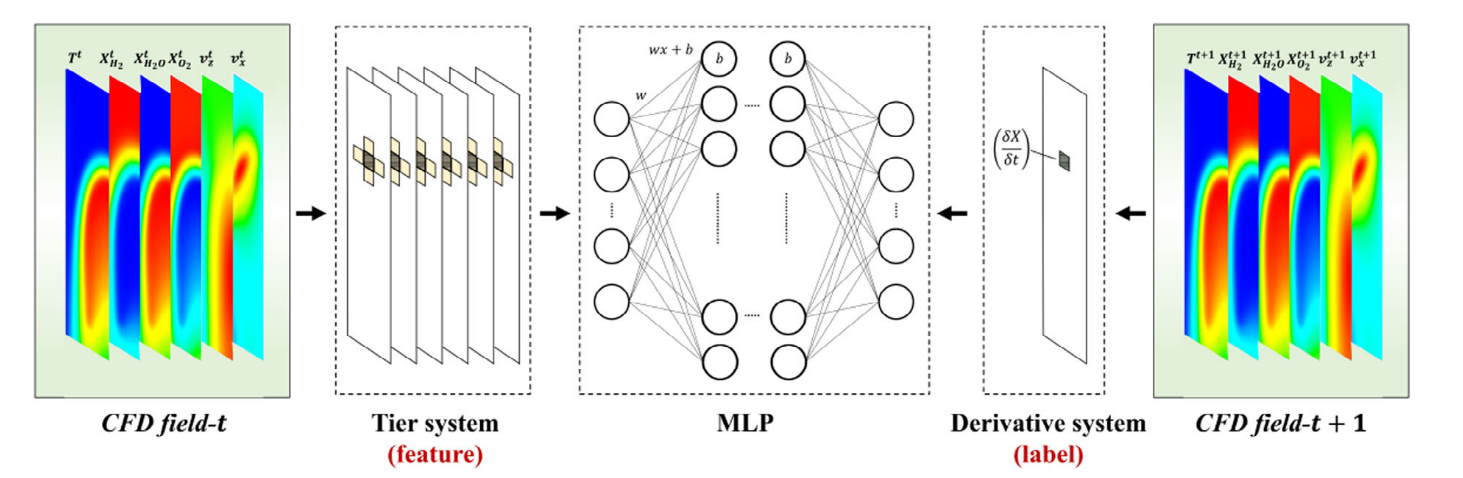
\includegraphics[width=1\linewidth]{figures//Literature review/FVMN.png}
    \caption{Overview of the FVMN architecture, showing the tier-derivative input/output system built around a conventional FFN (or MLP), adapted from \cite{Jeon2022}}
    \label{fig: FVMN}
\end{figure}

In the original work \textcite{Jeon2022}, significant improvements in accuracy were showcased compared to general models without the tier/derivative system implemented, where the authors managed to achieve a relative error with respect to CFD data of not more than 0.05\%, compared to 1.12\% for the conventional model.

In the context of accelerating CFD simulations, the FVMN also showed promising results. Due to the system's linearly increasing gradient error when used for longer transient predictions, the authors proposed an ML-CFD cross-coupling framework. The Residual-based Physics Informed Transfer learning strategy (RePIT) \cite{Jeon2024} is a hybrid framework where both a CFD solver and the FVMN alternately predict time series of fluid flows. RePIT continuously monitors the residuals of the governing equations, NSE \ref{eq: navier-stokes}, which are part of the physics-informed loss function employed by the FVMN in the case of fluid flows. \autoref{fig: RePIT} shows a schematic overview of the transfer learning framework, it shows that when the residuals of the loss function ($\varepsilon$) exceed a predefined tolerance ($\varepsilon_{th}$), the CFD solver will use the latest prediction and continue solving the governing equations to reduce the residuals back to a desired value. Afterwards, these newly computed CFD snapshots are used to update the network parameters, allowing for new predictions to be made. 

\begin{figure}[H]
    \centering
    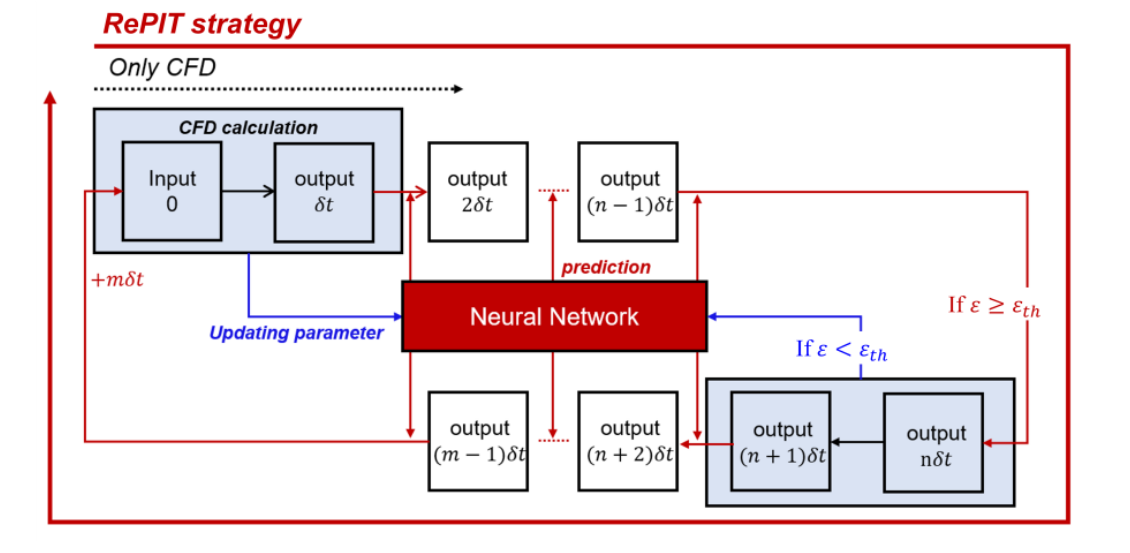
\includegraphics[width=1\linewidth]{figures//Literature review/RePIT.png}
    \caption{Schematic overview of the RePIT strategy showing the transfer learning process, adapted from \cite{Jeon2024}}
    \label{fig: RePIT}
\end{figure}

This framework leads to significant computational speed-ups without compromising accuracy. The authors implemented this method in a natural convection CFD case, achieving a 1.9 times acceleration, including network parameter updates. This demonstrates the strong capabilities of the FVMN, as its tier-based input system requires a minimal amount of training data. RePIT shows strong potential as it is universally adaptable to various flow cases and boundary conditions. 

While RePIT and FVMNs approximate spatial derivatives using mesh-based network structures, they can achieve smoother predictions by enabling the functionality of a continuous integrator, such as NODEs. Embedding NODEs into the RePIT framework would merge its residual-based transfer learning with NODEs’ ability to handle adaptive time integration and irregular sampling. This combination has the potential to enhance stability, improve generalisation across flow regimes, and further reduce the computational cost of turbulent CFD simulations

\pagebreak

\subsection{Challenges and Future Directions}

Machine learning has presented interesting solution paradigms for accelerating CFD simulations across various fronts. The most promising direction is the development of hybrid ML-CFD methods. Where traditional CFD solvers and ML models alternate between calculating/predicting time series data, methods like RePIT \cite{Jeon2024} and CFDNet \cite{Obiols-Sales2020} demonstrate that, when training data and loss functions are controlled, error accumulation can be mitigated, yielding significant speedups. Their online operation also enables the transferability of hybrid methods to a range of flow cases, making them more applicable to real-world CFD workflows. 

The ML-enhanced CFD field is also showing promising advances through more sophisticated architectures and loss functions. Frameworks such as PINNs \cite{Raissi2019} and PNODEs \cite{Sholokhov2023} can enforce physical constraints, such as incompressibility, and learn from observational data to provide accurate predictions of complex flow fields. It can therefore be argued that the embedding of physical laws into neural network architecture is an essential feature for future acceleration frameworks.

Despite these advancements, key challenges and opportunities remain in the field. One of these is the interpretability of the ML models. Due to their often complex nature, ML models tend to be a black box model. This opaqueness hinders their performance as effectively as physics-based models, making it difficult to understand why a model made a specific prediction \cite{Vinuesa2022, Girimaji2024}. This is a critical issue for generalisation, as models trained solely on data may struggle with unseen geometries and flow conditions, or when extrapolating beyond the training data's probability distribution. While advancements in hardware architecture \cite{ansys2023multiGPU, Chen2009} and automatic data generation continue to aid in providing the high-quality datasets needed for these models, the ultimate goal is to enable ML to not only accelerate simulations but also advance discoveries of new physical mechanisms and revisit empirical laws in fluid mechanics through more transparent and quantifiable models. 

While efforts continue for automatic data generation and automated experimentation pipelines to provide the large, high-quality datasets needed, the ultimate goal is to enable ML to not only accelerate simulations but also to assist in discovering new physical mechanisms and revisiting existing empirical laws in fluid mechanics, by yielding more transparent and certifiable models \cite{Brunton2020, Vinuesa2022}.

Despite the numerous advancements made in applying machine learning to CFD, the current literature still reveals several limitations. Many studies have employed NODEs only within reduced-order models \cite{Rojas2021, Shankar2022}, rather than integrating them directly into the CFD solver to accelerate the core time-integration step. Notably, their ability to serve as continuous time integrators has not been fully leveraged in scale-resolved simulations. That is why this work proposes applying a similar method to the RePIT framework by replacing its FVMN with NODEs. The RePIT framework showed that long-term stable acceleration can be achieved by alternating between CFD and machine learning predictions, guided by residual monitoring of the governing equations. The implementation of NODEs into the RePIT strategy can thus leverage RePIT’s residual-based transfer learning, complemented by NODEs’ continuous-time formulation. This strategy aims to directly address the bottleneck of time integration in CFD solvers, while ensuring that physical consistency is maintained through the use of residual monitoring. By pursuing this integration, the framework seeks to provide a concrete answer to the research questions introduced earlier: whether NODEs can deliver solver-level acceleration without compromising accuracy, and how residual monitoring can make such integration feasible.
% \todo{herschrijven}